\documentclass[10pt,xcolor=dvipsnames]{beamer}

\usetheme{CambridgeUS}
\usepackage[utf8x]{inputenc}
\usepackage{default}
\usepackage{graphicx}
\usepackage{epstopdf}
\usepackage{color}
\usepackage{amssymb,amsmath,amsfonts}
\usepackage{tikz}
\usepackage{siunitx}

\setbeamertemplate{navigation symbols}{}
\setbeamertemplate{itemize items}[square]
\setbeamertemplate{itemize subitem}[triangle]
\setbeamercolor{itemize item}{fg=darkred!80!gray}
\setbeamercolor{itemize subitem}{fg=darkred!80!gray}
\setbeamertemplate{title page}[default][colsep=-4bp,rounded=true]
\setbeamertemplate{blocks}[default]
\setbeamercolor{block title}{bg=darkred!80!black,fg=white}
\setbeamercolor{block body}{bg=gray!15!white,fg=black}

\setbeamercolor{blank}{bg=white,fg=white}
\setbeamercolor{note}{fg=white,bg=darkred!80!black}

\newenvironment<>{emphblock}{
 \begin{actionenv}%
  \def\insertblocktitle{\vspace{-1.25ex}}
  \par
  \mode<presentation>{
   \setbeamercolor{block title}{}
   \setbeamercolor{block body}{fg=white,bg=darkred!80!black}
   \setbeamercolor{itemize item}{fg=white,bg=darkred!80!black}
   \setbeamertemplate{itemize item}[square]
  }
  \usebeamertemplate{block begin}}
 {\par\usebeamertemplate{block end}\end{actionenv}
}

\title[Pedestal Structure and Stability]{Pedestal Structure and Stability in High-Performance Plasmas on Alcator C-Mod\\\vspace{-1em}}
\author[JR Walk]{John Walk}
\institute[MIT PSFC]{MIT Plasma Science and Fusion Center}
\date[7/22/14]{Thesis Defense -- 22 July 2014}

\graphicspath{{/home/jrwalk/Documents/CMod/common_graphics/}{E:/Libraries/Documents/Schoolwork/graphics/}}

\begin{document}

%%%%%%%%%%%%%%%%%%%%%%%%%%%%%%%%%%%%%%%%%%%%%%%%%%%%%%%%%%%%%%%%%%%%%

\begin{frame}

 \titlepage
 \begin{tikzpicture}[overlay]
  \node[anchor=east,xshift=-2ex,yshift=3ex] at (current page.south east) {\includegraphics[height=2cm]{cmodlogo.eps}};
 \end{tikzpicture}
 
\end{frame}

%%%%%%%%%%%%%%%%%%%%%%%%%%%%%%%%%%%%%%%%%%%%%%%%%%%%%%%%%%%%%%%%%%%%%

\begin{frame}{Thank you to...}

\large
\begin{itemize}
 \item The thesis committee: JW Hughes, DG Whyte, AE White, JP Freidberg
 \vspace{0.5em}
 \item The I-mode crew: AE Hubbard, JL Terry, I Cziegler, A Dominguez, SG Baek, C Theiler, RM Churchill, ML Reinke, JE Rice...
 \vspace{0.5em}
 \item Physops: R Granetz, S Shiraiwa, S Wolfe, S Wukitch...
 \vspace{0.5em}
 \item C-Mod operations, engineering, researchers and techs
 \vspace{0.5em}
 \item PSFC grad students, past and present
 \vspace{0.5em}
 \item Family and friends
 \vspace{0.5em}
 \item the audience!
\end{itemize}

\end{frame}

%%%%%%%%%%%%%%%%%%%%%%%%%%%%%%%%%%%%%%%%%%%%%%%%%%%%%%%%%%%%%%%%%%%%%

\begin{frame}{Outline}

\only<1>{\begin{itemize}
 \large
 \item \textbf{Context \& Motivation}
 \begin{itemize}
  \large 
  \item High-performance regimes
  \item Pedestal physics
  \item Introduction to I-mode
 \end{itemize}
 \vspace{0.5em}
 \item \textbf{Pedestal Modeling \& Theory}:
 \begin{itemize}
  \large
  \item Peeling-ballooning MHD stability
  \item Kinetic-ballooning mode turbulence
 \end{itemize}
 \vspace{0.5em}
 \item \textbf{ELMy H-Mode Physics}\footnote{JR Walk \emph{et al.}, \emph{Nuclear Fusion} \textbf{52} (2012)}
 \begin{itemize}
  \large
  \item EPED Modeling on C-Mod
 \end{itemize}
\end{itemize}}

\only<2->{\begin{itemize}
 \large
 \item \textbf{I-Mode Pedestals \& Global Performance}\footnote[2]{JR Walk \emph{et al.}, \emph{Physics of Plasmas} \textbf{21} (2014)}$^,$\footnote[3]{\emph{Invited talk}, APS-DPP Nov. 2013}
 \begin{itemize}
  \large
  \item Pedestal response to fueling, heating power
  \item Pedestal widths and gradients
  \item Global performance and confinement scalings
 \end{itemize}
 \vspace{0.5em}
 \item \textbf{I-Mode Pedestal Stability}
 \begin{itemize}
  \large
  \item P-B MHD, KBM modeling
  \item ELM characterization
 \end{itemize}
 \vspace{0.5em}
 \item \textbf{Summary, Future Work, \& Questions}
\end{itemize}}

\end{frame}

%%%%%%%%%%%%%%%%%%%%%%%%%%%%%%%%%%%%%%%%%%%%%%%%%%%%%%%%%%%%%%%%%%%%%

\begin{frame}{The problem...}

 \large
 By default (``L-mode''), rapid transport of energy and particles from plasma driven by turbulence
 
 \begin{itemize}
  \item and energy transport gets \emph{worse} with more heating power!
  \item need very strong magnetic field and/or large machine size to overcome poor plasma performance
 \end{itemize}
 
\begin{emphblock}{}
  \centering
  L-mode likely not suitable for (economical) power plant development.
 \end{emphblock}

\end{frame}

%%%%%%%%%%%%%%%%%%%%%%%%%%%%%%%%%%%%%%%%%%%%%%%%%%%%%%%%%%%%%%%%%%%%%

\begin{frame}{The solution?}
 \large
 Under right conditions, plasma forms ``transport barrier'' in edge, with steep gradients in density and temperature -- the \emph{pedestal}
 
 $\rightarrow$ plasma transitions to ``high-confinement'' or H-mode
 
 \begin{itemize}
  \item immediate factor of $\sim 2$ increase in energy confinement
  \item pedestal supports higher core pressures $=$ fusion power density
 \end{itemize}
 
 \begin{emphblock}{}
  \centering
  pedestal height sets strong constraint on global performance
 \end{emphblock}

\end{frame}

%%%%%%%%%%%%%%%%%%%%%%%%%%%%%%%%%%%%%%%%%%%%%%%%%%%%%%%%%%%%%%%%%%%%%

\begin{frame}{...But this has problems of its own}

 \begin{columns}[c]
  \column{0.5\textwidth}
  \vspace{-2em}
  \begin{itemize}
   \large
   \item increased particle confinement $=$ plasma retains impurities as well as fuel ions
   \vspace{0.5em}
   \item radiated power ($\sim Z^2$ for a given impurity species) increases, overcomes heating power $\rightarrow$ plasma drops back into L-mode
   \vspace{0.5em}
   \item \textcolor{red}{inherently transient state}
  \end{itemize}
  \column{0.5\textwidth}
  \centering
  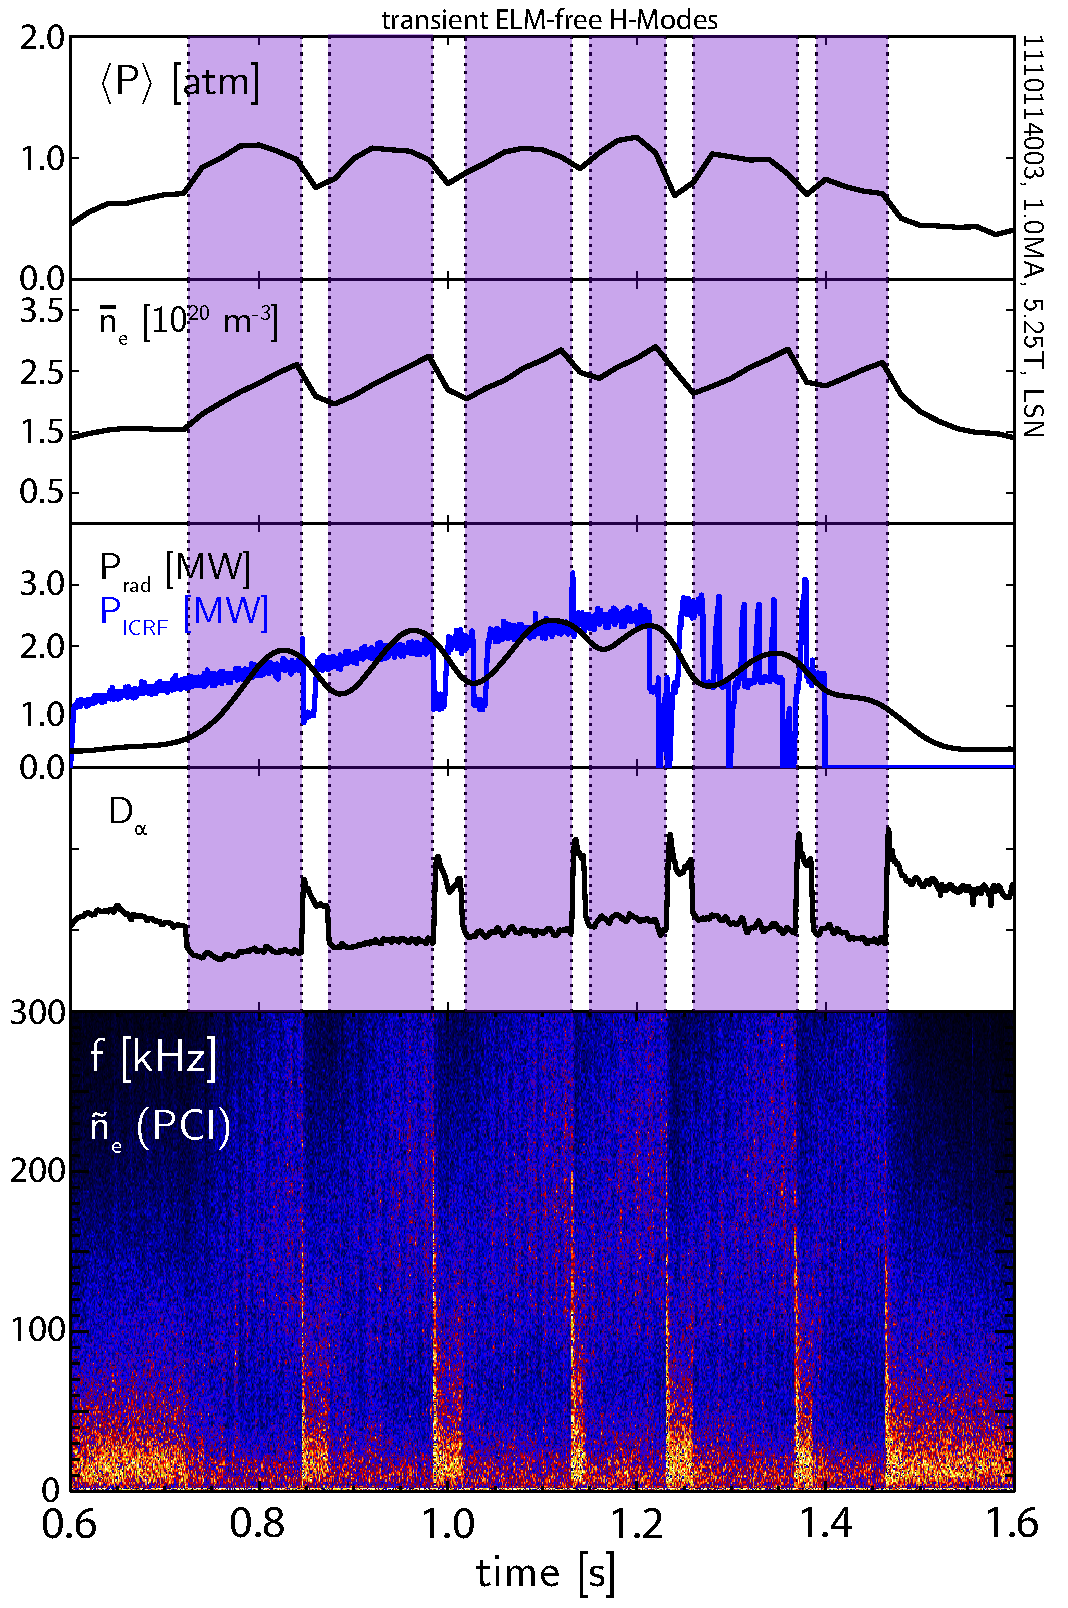
\includegraphics[width=0.85\columnwidth]{graphics/HighPerformanceRegimes/trace_1110114003.pdf}
 \end{columns}

\end{frame}

%%%%%%%%%%%%%%%%%%%%%%%%%%%%%%%%%%%%%%%%%%%%%%%%%%%%%%%%%%%%%%%%%%%%%

\begin{frame}

\Large
so, we need:
\begin{itemize}
 \item high energy confinement
 \item low particle confinement (low enough, at least)
 \item ... and that's it, right?
\end{itemize}

\end{frame}

%%%%%%%%%%%%%%%%%%%%%%%%%%%%%%%%%%%%%%%%%%%%%%%%%%%%%%%%%%%%%%%%%%%%%

\begin{frame}{The solution? (part II)}

 \begin{columns}[c]
  \column{0.5\textwidth}
  \begin{itemize}
   \large
   \item Edge-Localized Modes (ELMs) -- instabilities that relax the pedestal, drive bursts of energy, particle transport, enough to prevent impurity accumulation
   \vspace{0.5em}
   \onslide<2>{\item \textcolor{red}{large ELMs drive pulsed heat loads in excess of plasma-facing material tolerances}}
  \end{itemize}
  \column{0.5\textwidth}
  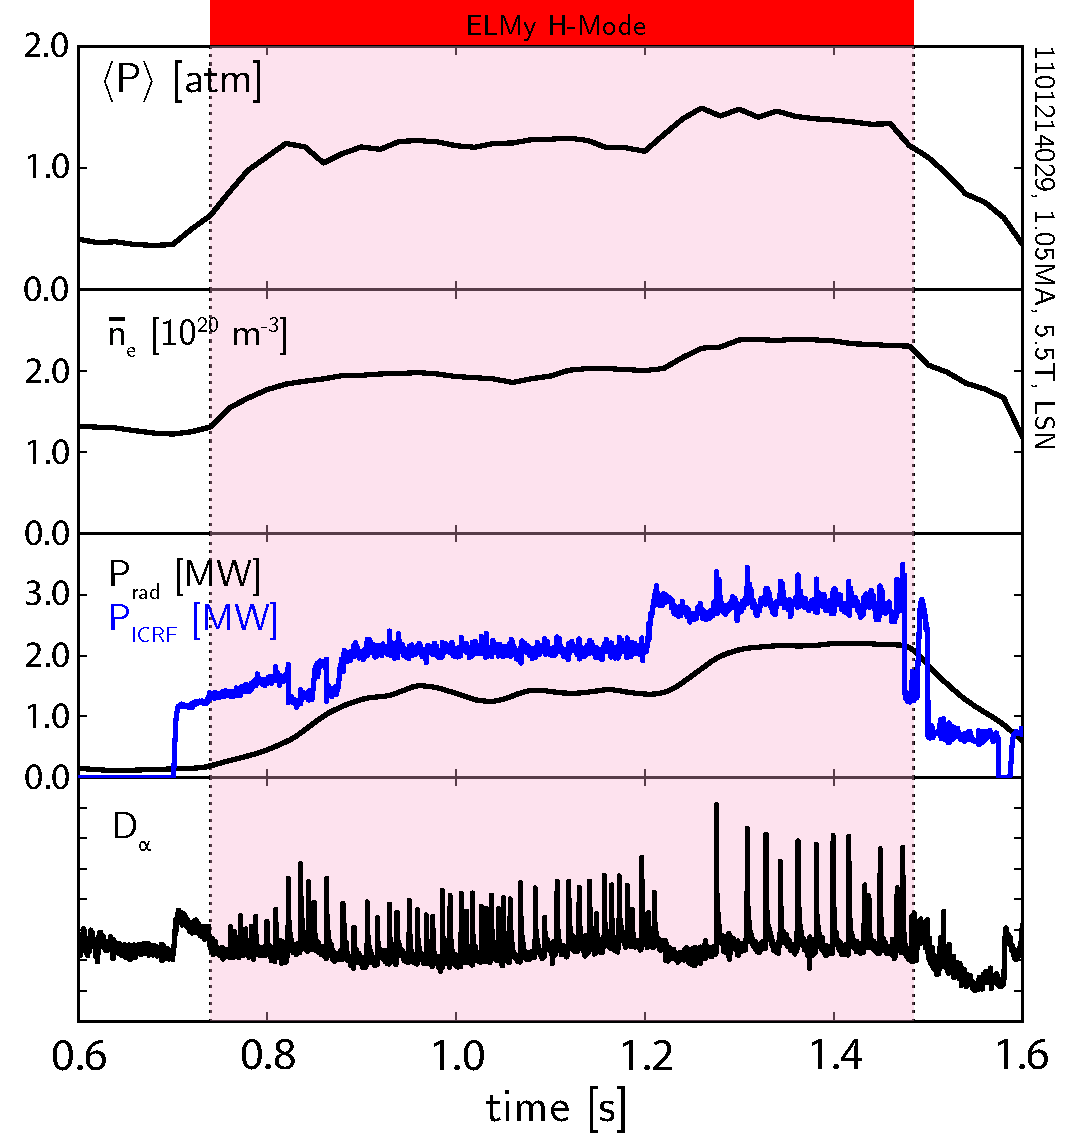
\includegraphics[width=\columnwidth]{graphics/HighPerformanceRegimes/trace_1101214029.pdf}
 \end{columns}

\end{frame}

%%%%%%%%%%%%%%%%%%%%%%%%%%%%%%%%%%%%%%%%%%%%%%%%%%%%%%%%%%%%%%%%%%%%%

\begin{frame}

\Large
so, we need:
\begin{itemize}
 \item high energy confinement
 \item low particle confinement (low enough, at least)
 \item avoid, mitigate, or suppress large ELMs
 \onslide<2->{\begin{itemize}
  \large
  \onslide<3->{\item engineering solutions:\\ pellet pacing, resonant magnetic perturbations}
  \onslide<4>{\item physics solutions:\\ pedestal regulation by fluctuations below ELM limit}
 \end{itemize}}
\end{itemize}

 \only<2>{\begin{tikzpicture}[overlay]
  \node[anchor=north,yshift=-9ex,xshift=-2ex] at (current page.center) {
\includegraphics[height=4cm]{graphics/Other/spanishinquisition.jpeg}};
 \end{tikzpicture}}

\end{frame}

%%%%%%%%%%%%%%%%%%%%%%%%%%%%%%%%%%%%%%%%%%%%%%%%%%%%%%%%%%%%%%%%%%%%%

\begin{frame}{The solution? (part III)}

\large
A number of fluctuation-regulated regimes have been observed:
\vspace{0.5em}
\begin{itemize}
 \large
 \item EDA H-mode\\ Quasi-Coherent Mode (QCM) -- C-Mod, AUG(?)
 \item Quiescent H-mode\\ Edge Harmonic Oscillator (EHO) -- DIII-D, JET, AUG
 \item High-Recycling Steady H-mode\\ edge MHD fluctuations -- JFT-2M
 \item type-II, -III ELMy H-modes\\ small, rapid ELMs -- various devices
\end{itemize}

\vspace{0.5em}
generally capable of stationary high performance without large ELMs

\end{frame}

%%%%%%%%%%%%%%%%%%%%%%%%%%%%%%%%%%%%%%%%%%%%%%%%%%%%%%%%%%%%%%%%%%%%%

\begin{frame}{EDA H-mode (on C-Mod and elsewhere)}

\begin{columns}[c]
 \column{0.5\textwidth}
  \vspace{-2em}
  \begin{itemize}
   \large
   \item pedestal regulated by continuous edge fluctuation (QCM), rather than bursts of ELM transport
   \vspace{0.5em}
   \item steady density, $P_{rad} = $ stationary operation possible with good performance
  \end{itemize}
 \column{0.5\textwidth}
  \centering
  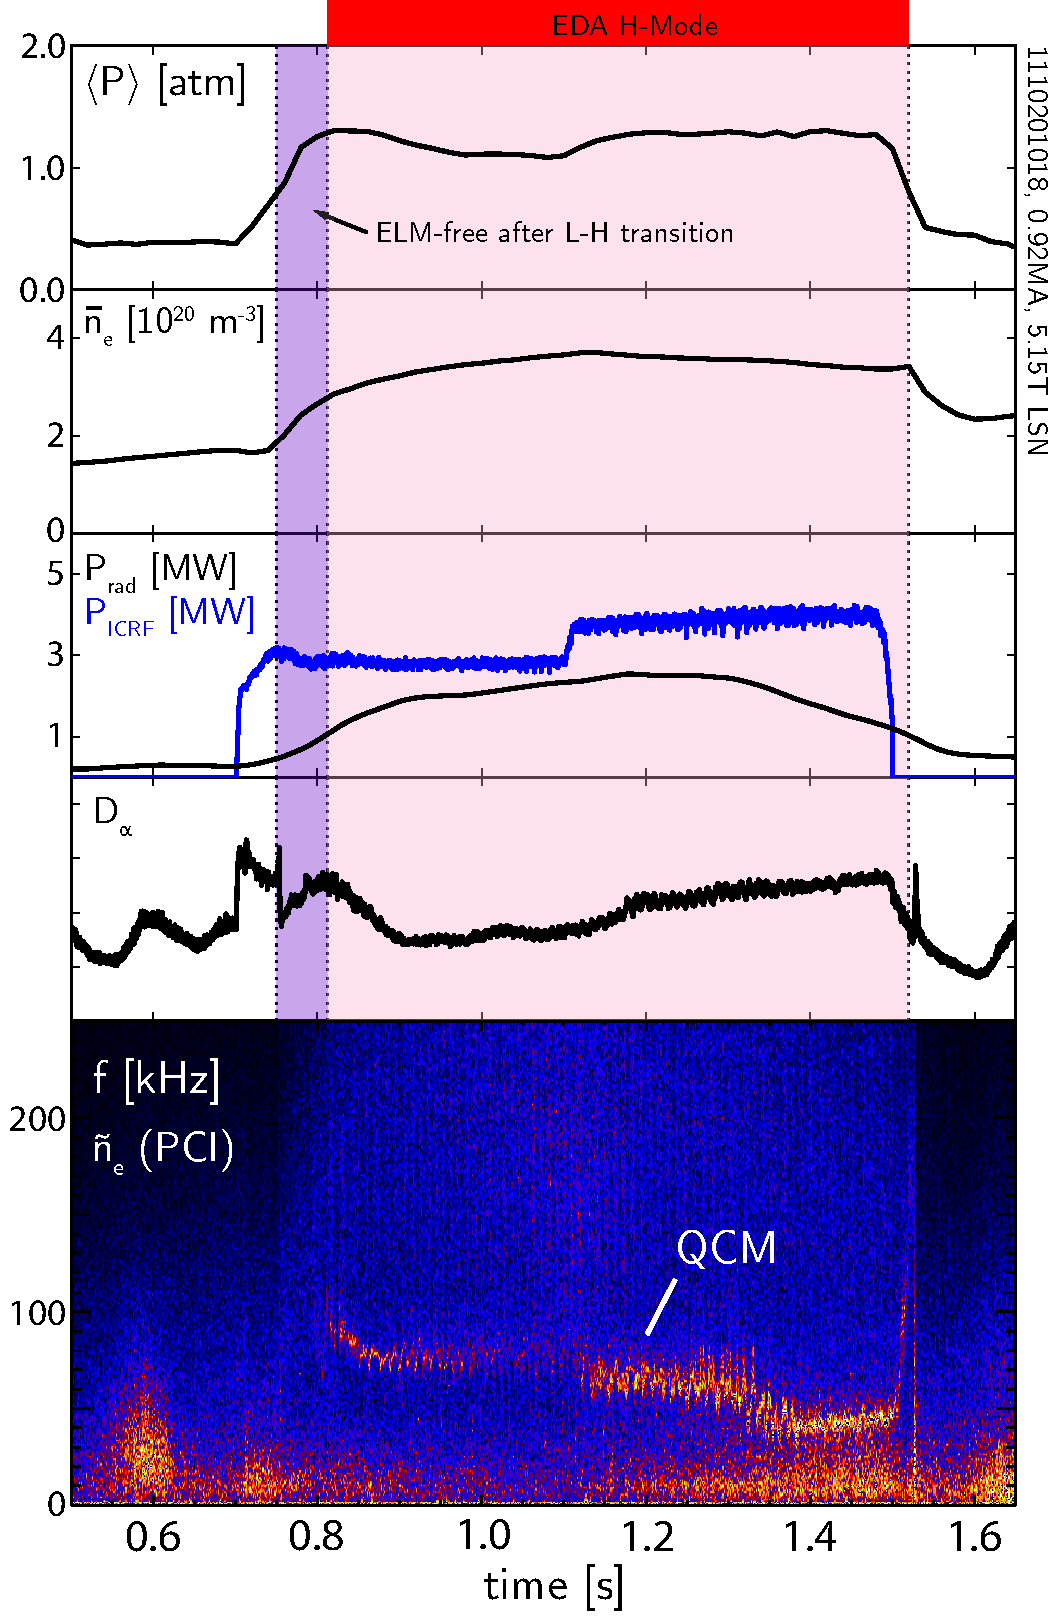
\includegraphics[width=0.85\columnwidth]{graphics/HighPerformanceRegimes/trace_1110201018.pdf}
\end{columns}

\end{frame}

%%%%%%%%%%%%%%%%%%%%%%%%%%%%%%%%%%%%%%%%%%%%%%%%%%%%%%%%%%%%%%%%%%%%%

\begin{frame}{But each of these has drawbacks}

\large
\begin{itemize}
 \item engineering requirements, e.g. high beam torque for QH-mode
 \item access limits: high collisionality for EDA, shaping for type-II ELMs
\end{itemize}

\begin{emphblock}{}
  \centering
  Can we do better?
 \end{emphblock}

\end{frame}

%%%%%%%%%%%%%%%%%%%%%%%%%%%%%%%%%%%%%%%%%%%%%%%%%%%%%%%%%%%%%%%%%%%%%

\begin{frame}{A challenger appears: the I-mode}

\centering
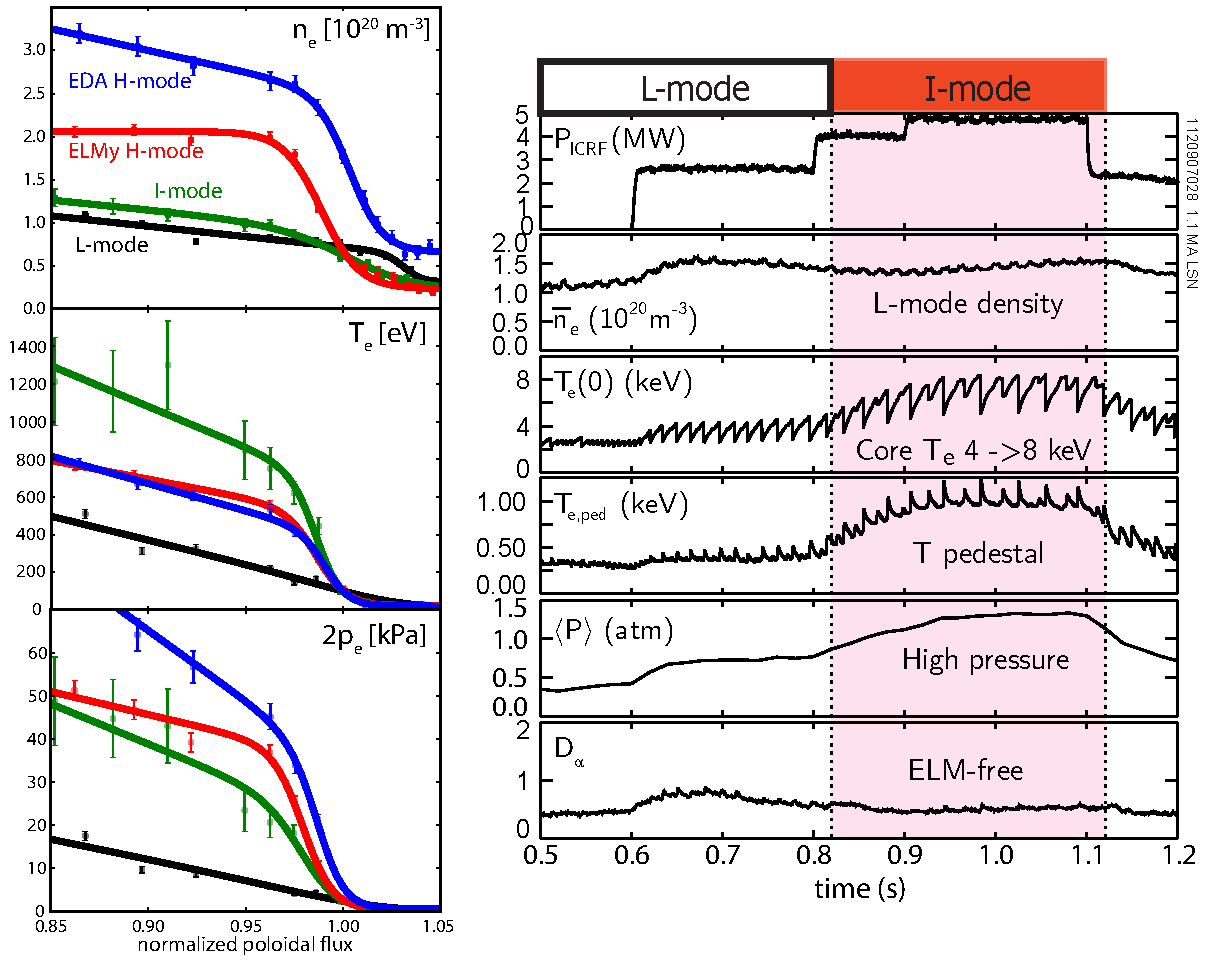
\includegraphics[width=0.8\textwidth]{graphics/HighPerformanceRegimes/trace_imode.pdf}

\end{frame}

%%%%%%%%%%%%%%%%%%%%%%%%%%%%%%%%%%%%%%%%%%%%%%%%%%%%%%%%%%%%%%%%%%%%%

\begin{frame}{I-mode pedestal regulated by\\ Weakly-Coherent Mode (WCM)}

 \centering
 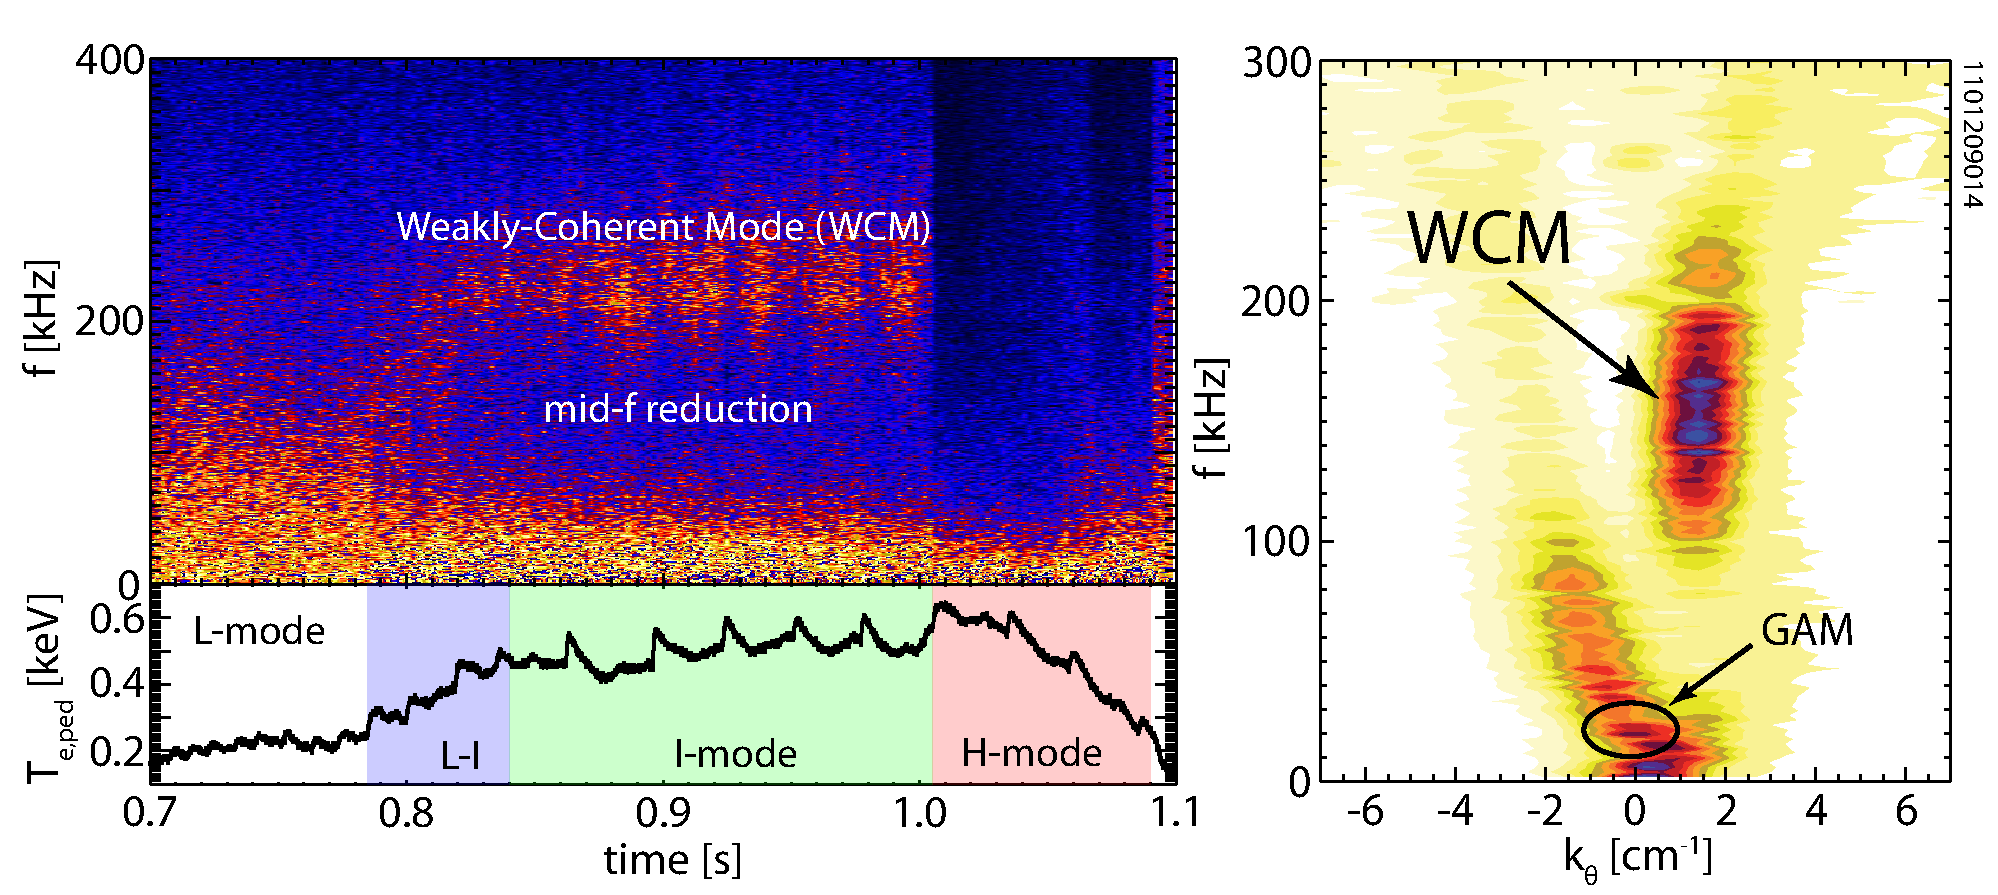
\includegraphics[width=\textwidth]{graphics/HighPerformanceRegimes/WCM.pdf}

\end{frame}

%%%%%%%%%%%%%%%%%%%%%%%%%%%%%%%%%%%%%%%%%%%%%%%%%%%%%%%%%%%%%%%%%%%%%

\begin{frame}{Robust I-mode access on C-Mod}

 \begin{columns}[c]
  \column{0.5\textwidth}
   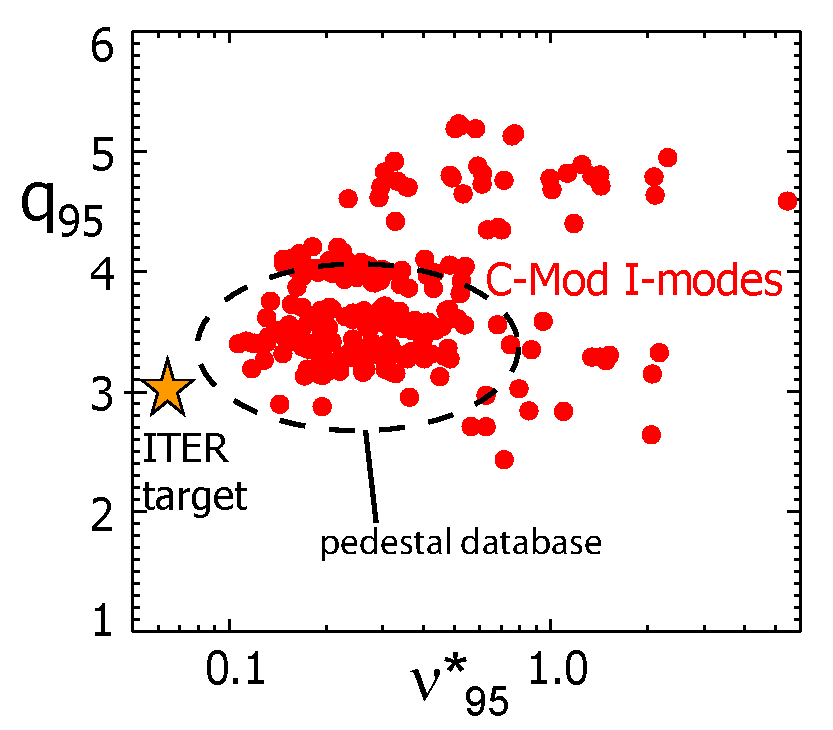
\includegraphics[width=\columnwidth]{graphics/IModePedestal/q95_vs_nustar_2012_Imodeonly.pdf}
  \column{0.5\textwidth}
   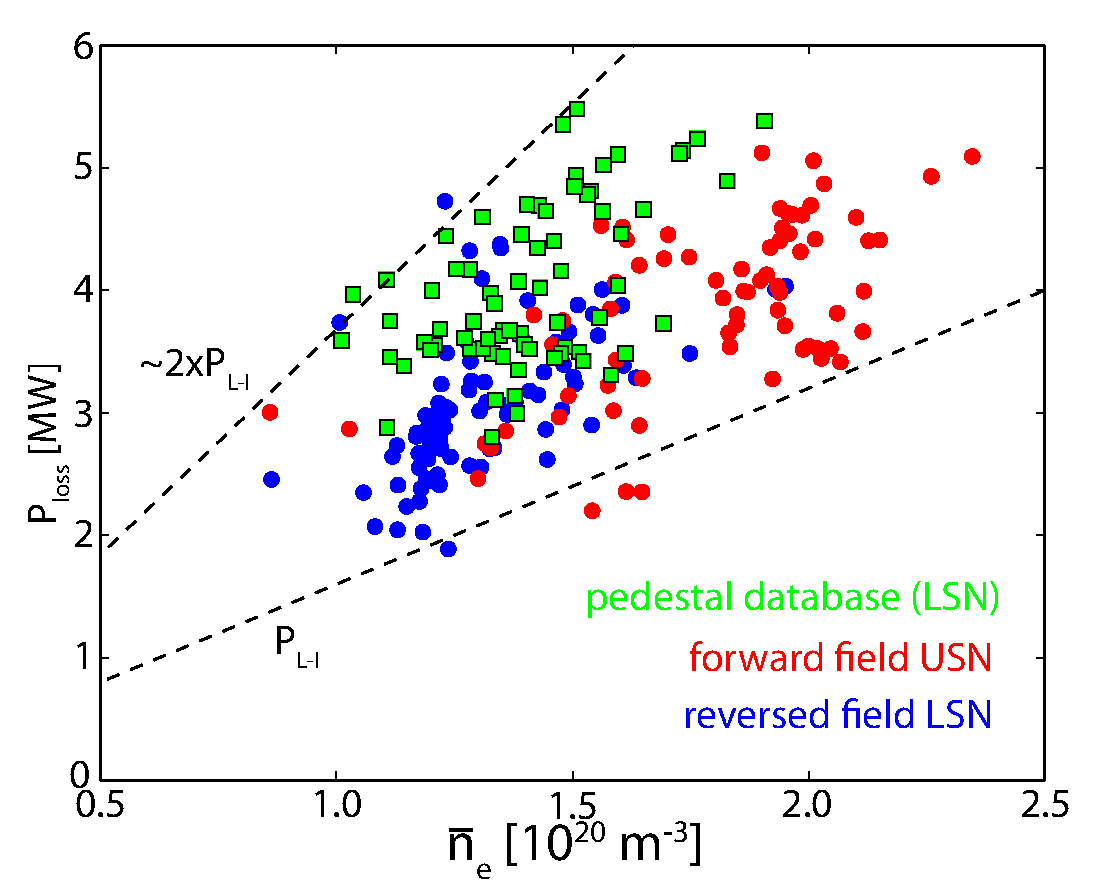
\includegraphics[width=\columnwidth]{graphics/IModePedestal/nebar_Ploss_all.pdf}
 \end{columns}
 
 \begin{itemize}
  \item I-mode accessed over range of edge current profiles, low-mid collisionalities
  \item ``Unfavorable'' $\nabla B$ orientation (ion $\nabla B$ drift away from primary X-point) -- forward-field upper-null or reversed-field lower-null operation
  \item Sustain mode with heating power up to $\sim 2\times$ above L-I threshold
 \end{itemize}

\end{frame}

%%%%%%%%%%%%%%%%%%%%%%%%%%%%%%%%%%%%%%%%%%%%%%%%%%%%%%%%%%%%%%%%%%%%%

\begin{frame}{Outline}

 \setbeamercolor{normal text}{fg=gray,bg=}
 \setbeamercolor{alerted text}{fg=black,bg=}
 \usebeamercolor{normal text}

 \begin{itemize}
 \large
 \item \textbf{Context \& Motivation}
 \begin{itemize}
  \large 
  \item High-performance regimes
  \item Pedestal physics
  \item Introduction to I-mode
 \end{itemize}
 \vspace{0.5em}
 \alert<+>{\item \textbf{Pedestal Modeling \& Theory}:
 \begin{itemize}
  \large
  \item Peeling-ballooning MHD stability
  \item Kinetic-ballooning mode turbulence
 \end{itemize}}
 \vspace{0.5em}
 \item \textbf{ELMy H-Mode Physics}\footnote[1]{JR Walk \emph{et al.}, \emph{Nuclear Fusion} \textbf{52} (2012)}
 \begin{itemize}
  \large
  \item EPED Modeling on C-Mod
 \end{itemize}
\end{itemize}

\end{frame}

%%%%%%%%%%%%%%%%%%%%%%%%%%%%%%%%%%%%%%%%%%%%%%%%%%%%%%%%%%%%%%%%%%%%%

\begin{frame}
 
 \large
 \centering
 how much detail here for modeling, vs in extra slides?

\end{frame}

%%%%%%%%%%%%%%%%%%%%%%%%%%%%%%%%%%%%%%%%%%%%%%%%%%%%%%%%%%%%%%%%%%%%%

\begin{frame}{Predictive Model for ELMy H-modes -- EPED\footnote[4]{PB Snyder \emph{et al.}, \emph{Nuclear Fusion} \textbf{51} (2011)}}

 \begin{center}
  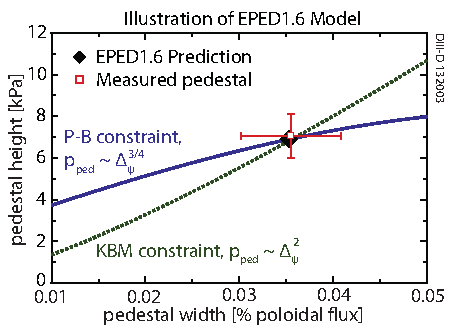
\includegraphics[width=0.8\columnwidth]{graphics/ModelingTheory/epedcartoon.pdf}
 \end{center}

\end{frame}

%%%%%%%%%%%%%%%%%%%%%%%%%%%%%%%%%%%%%%%%%%%%%%%%%%%%%%%%%%%%%%%%%%%%%

\begin{frame}{Pedestal Structure Definitions}

 \begin{columns}[c]
  \column{0.5\textwidth}
   \large
   pedestals fitted by
   \begin{align*}
    &z = \frac{x_0 - x}{\delta}\\
    &mtanh(\alpha,z) = \frac{(1 + \alpha z) e^{z} - e^{-z}}{e^{z} + e^{-z}}\\
    &y = \frac{h+b}{2} + \frac{h-b}{2} mtanh(\alpha,z)
   \end{align*}
  \column{0.5\textwidth}
   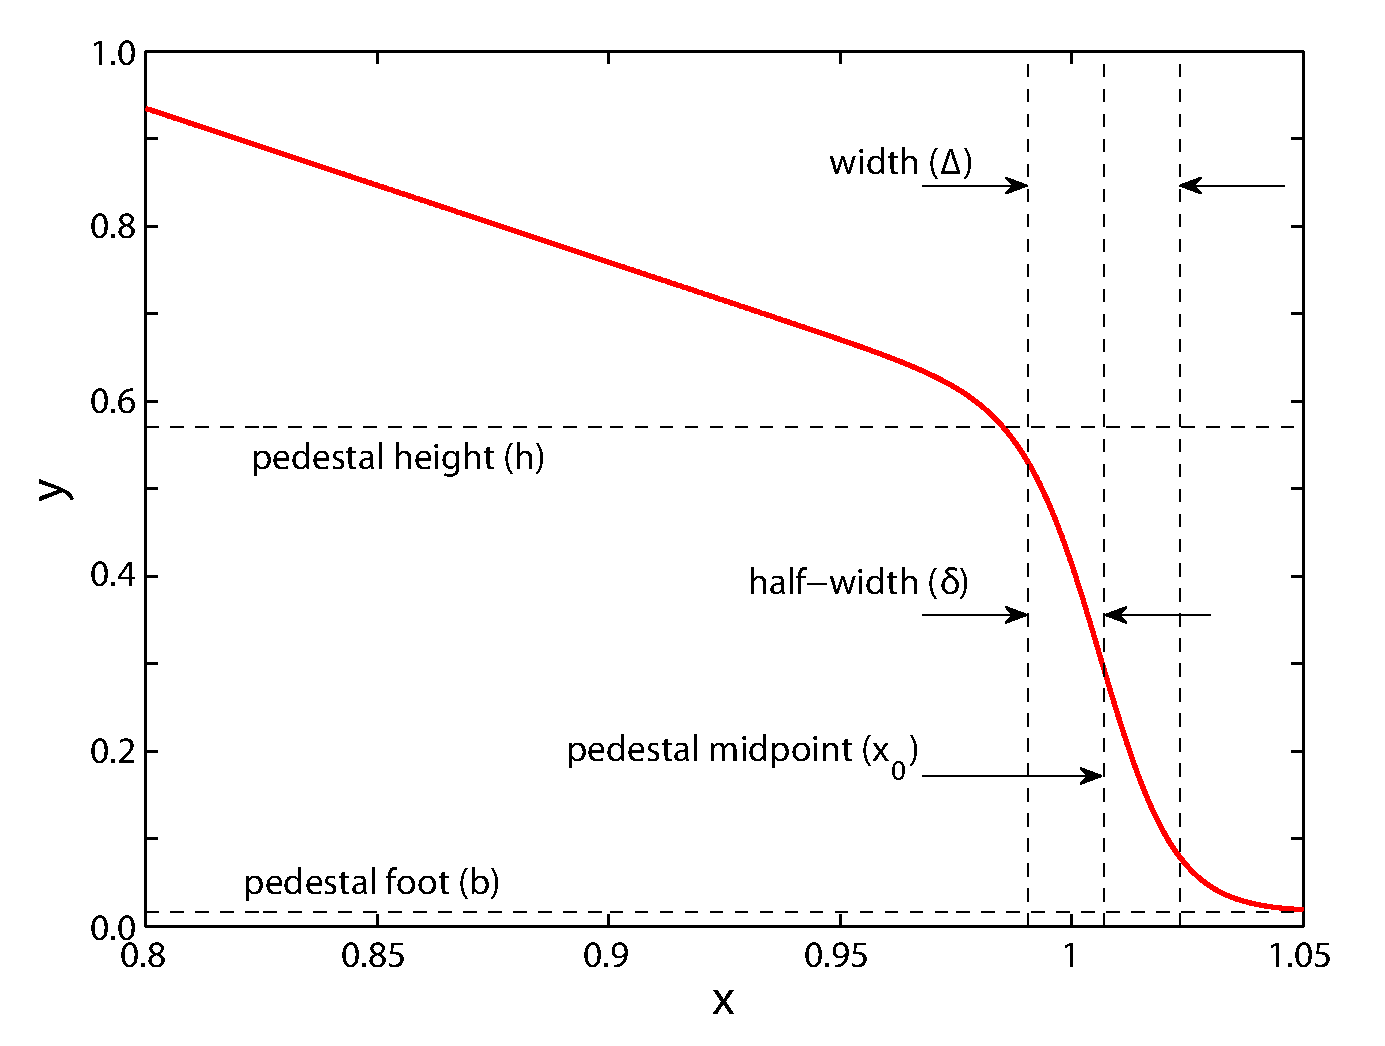
\includegraphics[width=\columnwidth]{graphics/ELMy/mtanh.pdf}
 \end{columns}
 
 \large
 \vspace{0.5em}
 rigorous definition for pedestal width $\Delta = 2\delta$, continuous and differentiable throughout pedestal profile

\end{frame}

%%%%%%%%%%%%%%%%%%%%%%%%%%%%%%%%%%%%%%%%%%%%%%%%%%%%%%%%%%%%%%%%%%%%%

\begin{frame}{Outline}

 \setbeamercolor{normal text}{fg=gray,bg=}
 \setbeamercolor{alerted text}{fg=black,bg=}
 \usebeamercolor{normal text}

 \begin{itemize}
 \large
 \item \textbf{Context \& Motivation}
 \begin{itemize}
  \large 
  \item High-performance regimes
  \item Pedestal physics
  \item Introduction to I-mode
 \end{itemize}
 \vspace{0.5em}
 \item \textbf{Pedestal Modeling \& Theory}:
 \begin{itemize}
  \large
  \item Peeling-ballooning MHD stability
  \item Kinetic-ballooning mode turbulence
 \end{itemize}
 \vspace{0.5em}
 \alert<+>{\item \textbf{ELMy H-Mode Physics}\footnote[1]{JR Walk \emph{et al.}, \emph{Nuclear Fusion} \textbf{52} (2012)}
 \begin{itemize}
  \large
  \item EPED Modeling on C-Mod
 \end{itemize}}
\end{itemize}

\end{frame}

%%%%%%%%%%%%%%%%%%%%%%%%%%%%%%%%%%%%%%%%%%%%%%%%%%%%%%%%%%%%%%%%%%%%%

\begin{frame}{Target steady ELMy phases for study}

 \centering
 
\includegraphics[width=\textwidth]{graphics/ELMy/time_window.pdf}

\end{frame}

%%%%%%%%%%%%%%%%%%%%%%%%%%%%%%%%%%%%%%%%%%%%%%%%%%%%%%%%%%%%%%%%%%%%%

\begin{frame}{ELM cycle binning necessary to capture pedestal limit}

 \begin{columns}[c]
  \column{0.5\textwidth}
   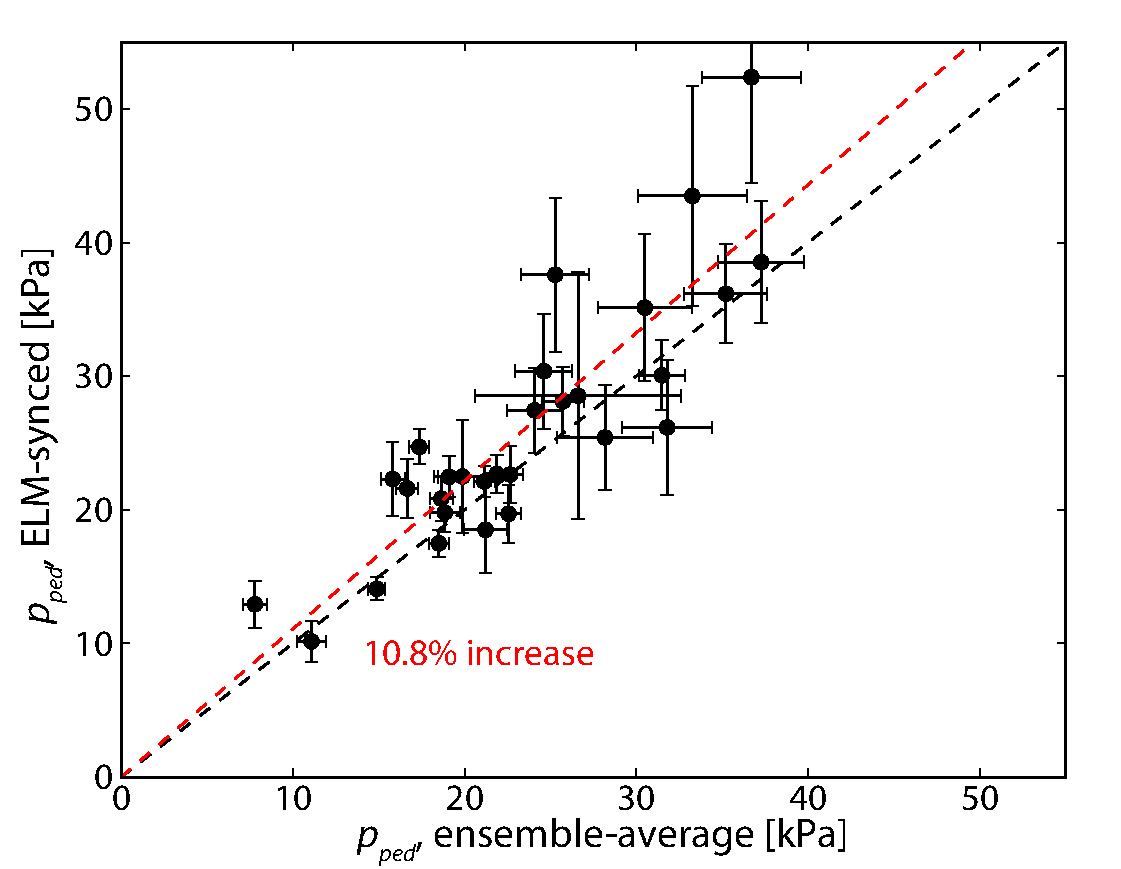
\includegraphics[width=\columnwidth]{graphics/ELMy/pped_ensemble_elmsync.pdf}
  \column{0.5\textwidth}
   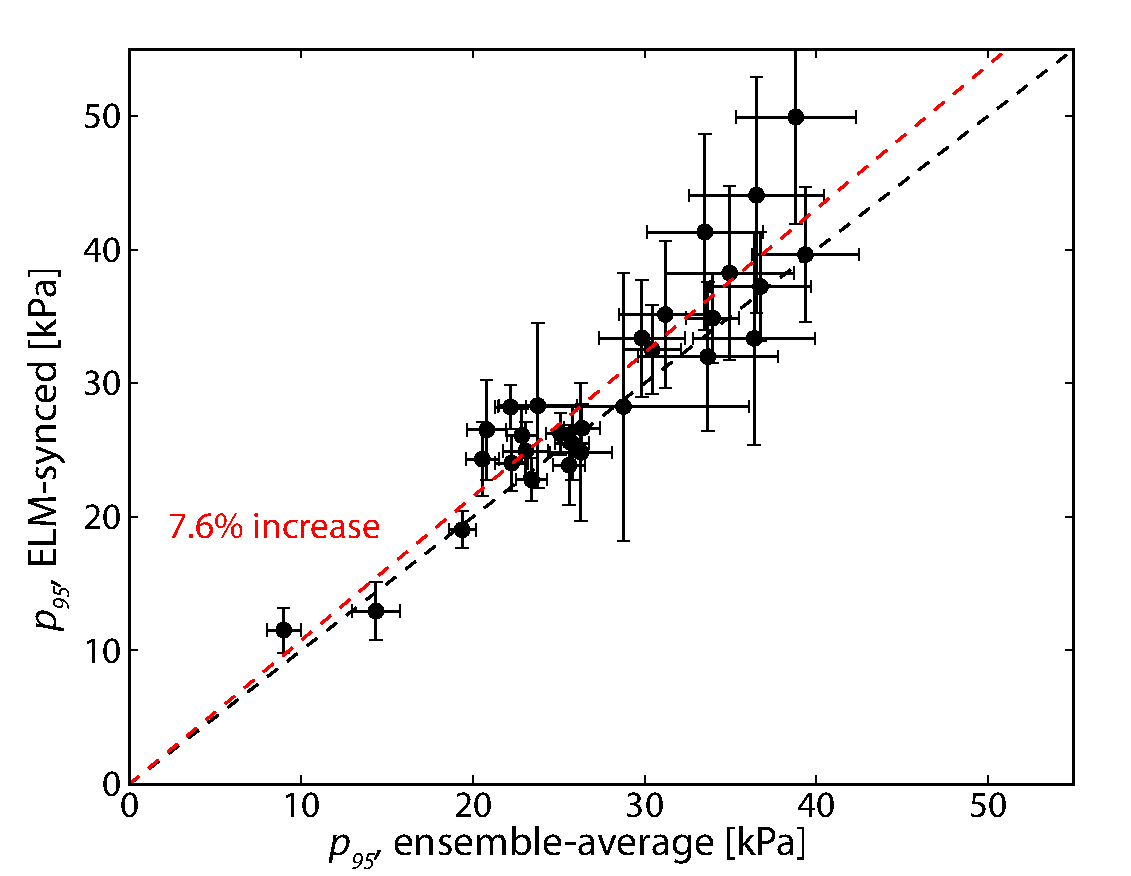
\includegraphics[width=\columnwidth]{graphics/ELMy/p95_ensemble_elmsync.pdf}
 \end{columns}
 
 \vspace{0.5em}
 Take profile data immediately preceding ELM crash (typically last 20\% of ELM cycle) for pedestal structure at point of instability -- necessary, but difficult given ELM frequency on C-Mod (subset of data prepared thus).

\end{frame}

%%%%%%%%%%%%%%%%%%%%%%%%%%%%%%%%%%%%%%%%%%%%%%%%%%%%%%%%%%%%%%%%%%%%%

\begin{frame}{Pedestal width described well by KBM limit}

 \centering
 \includegraphics<1>[width=0.65\textwidth]{graphics/ELMy/betap_deltapsi_all.pdf}
 \includegraphics<2>[width=0.65\textwidth]{graphics/ELMy/betap_deltapsi_elmsync.pdf}
 \includegraphics<3>[width=0.65\textwidth]{graphics/ELMy/betap_deltapsi_elmsync_betabin.pdf}
 
 \large
 KBM limit predicts width $\Delta_\psi = G(\nu^*,\varepsilon,...) \beta_{p,ped}^{1/2}$

\end{frame}

%%%%%%%%%%%%%%%%%%%%%%%%%%%%%%%%%%%%%%%%%%%%%%%%%%%%%%%%%%%%%%%%%%%%%

\begin{frame}{Minimal dependence of width on other parameters}

 

\end{frame}

%%%%%%%%%%%%%%%%%%%%%%%%%%%%%%%%%%%%%%%%%%%%%%%%%%%%%%%%%%%%%%%%%%%%%

\begin{frame}{Pedestal height predicted by ballooning $\nabla p$ limit}

 \begin{columns}[c]
  \column{0.5\textwidth}
   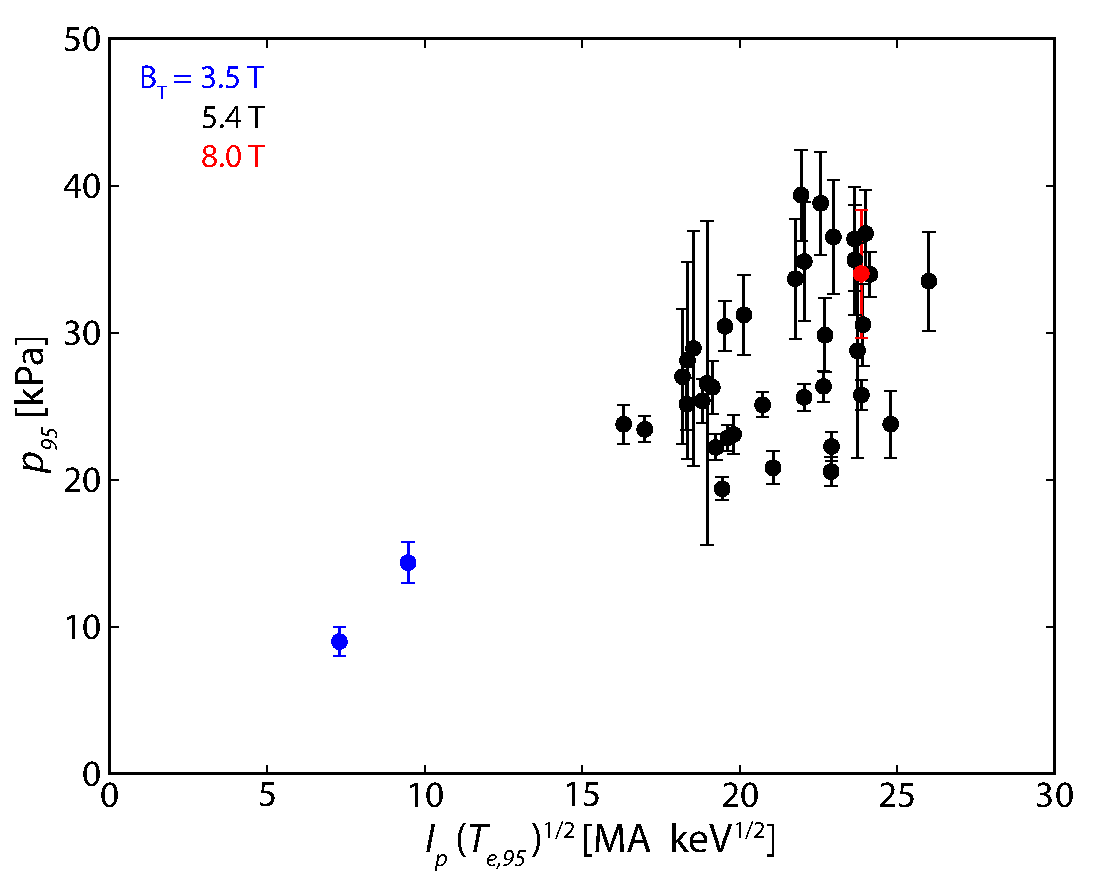
\includegraphics[width=\columnwidth]{graphics/ELMy/IprootTe_p95.pdf}
  \column{0.5\textwidth}
   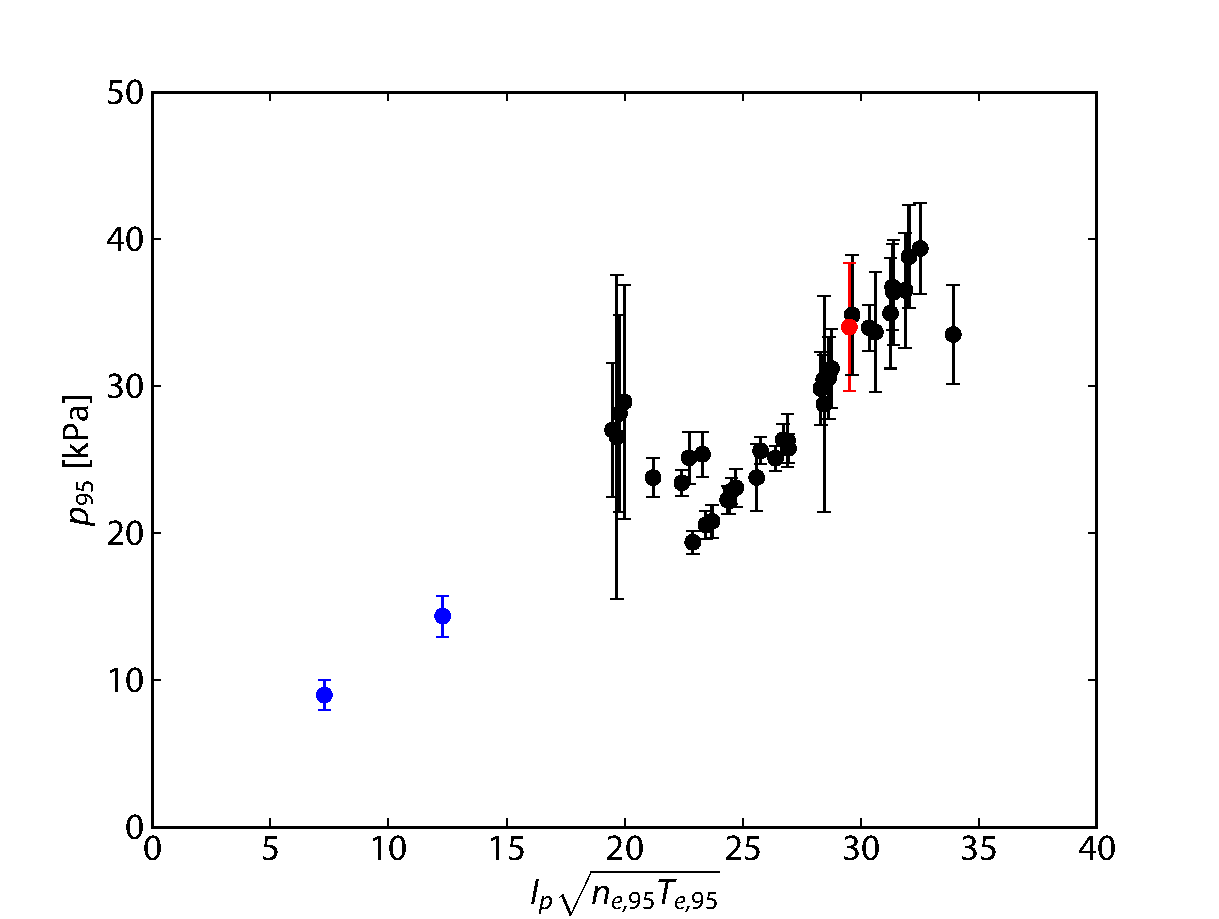
\includegraphics[width=\columnwidth]{graphics/ELMy/IprootneTe_p95.pdf}
 \end{columns}
 
 \large
 \vspace{0.5em}
 Pedestal height $p_{ped} \sim \nabla p \times \Delta_p \rightarrow \sim I_p^2 \Delta_p$ from ballooning MHD
 predicted well by $\Delta_p \sim \sqrt{\beta_{p,ped}}$, less so by $\Delta_p \sim \rho_{i,pol}$

\end{frame}

%%%%%%%%%%%%%%%%%%%%%%%%%%%%%%%%%%%%%%%%%%%%%%%%%%%%%%%%%%%%%%%%%%%%%

\begin{frame}{Robust width, gradient limit $=$ attainable $\beta_{p,ped}$\\ limited in ELMy H-mode}

 \begin{columns}[c]
  \column{0.5\textwidth}
   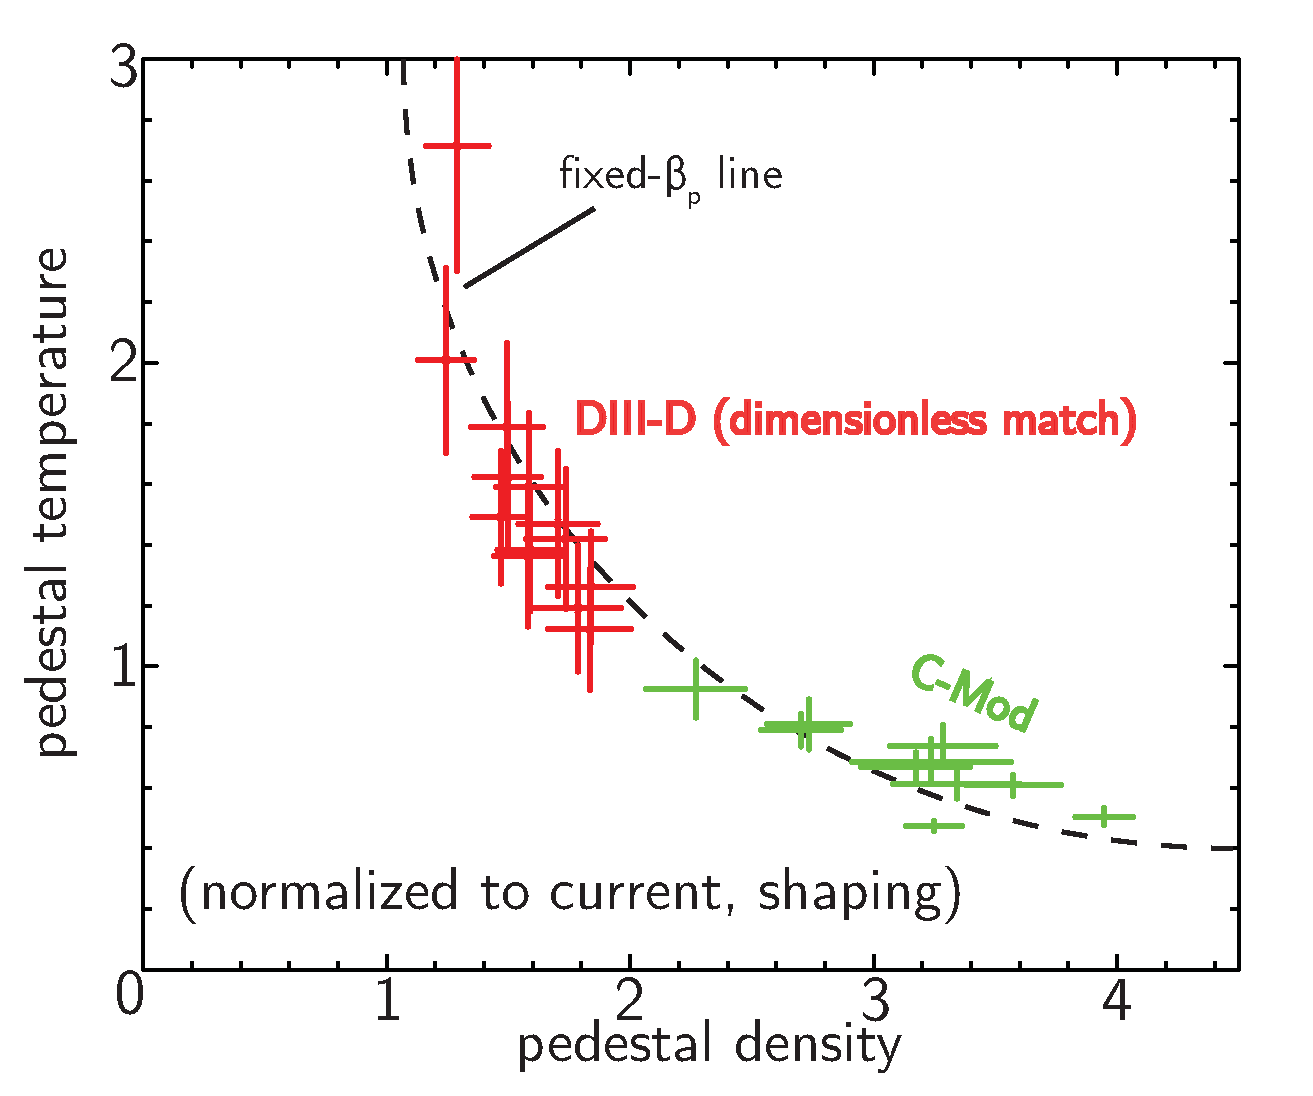
\includegraphics[width=\columnwidth]{graphics/HighPerformanceRegimes/elmy_betas.pdf}
  \column{0.5\textwidth}
   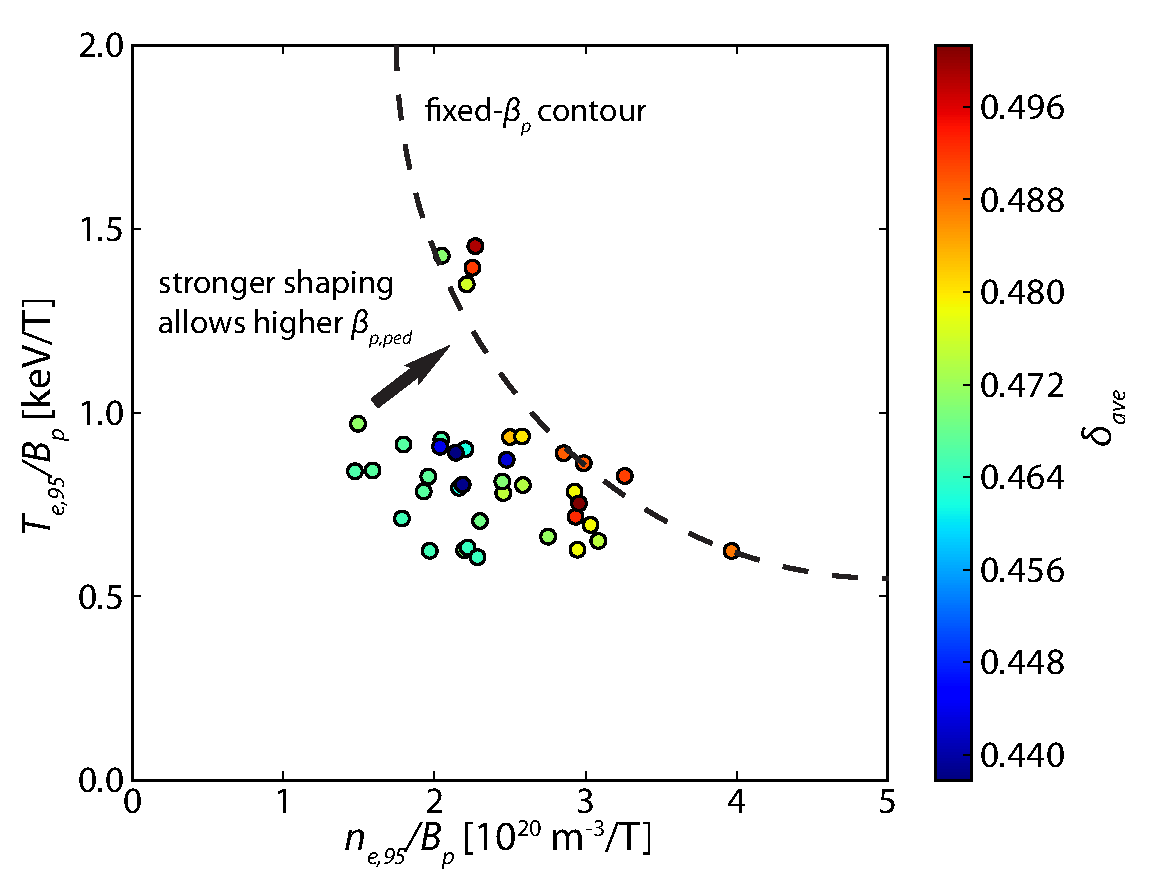
\includegraphics[width=\columnwidth]{graphics/ELMy/neBp_TeBp_deltaave.pdf}
 \end{columns}

\end{frame}

%%%%%%%%%%%%%%%%%%%%%%%%%%%%%%%%%%%%%%%%%%%%%%%%%%%%%%%%%%%%%%%%%%%%%

\begin{frame}{Computational modeling of P-B MHD,\\ KBM captures ELMy pedestal}

 \centering
 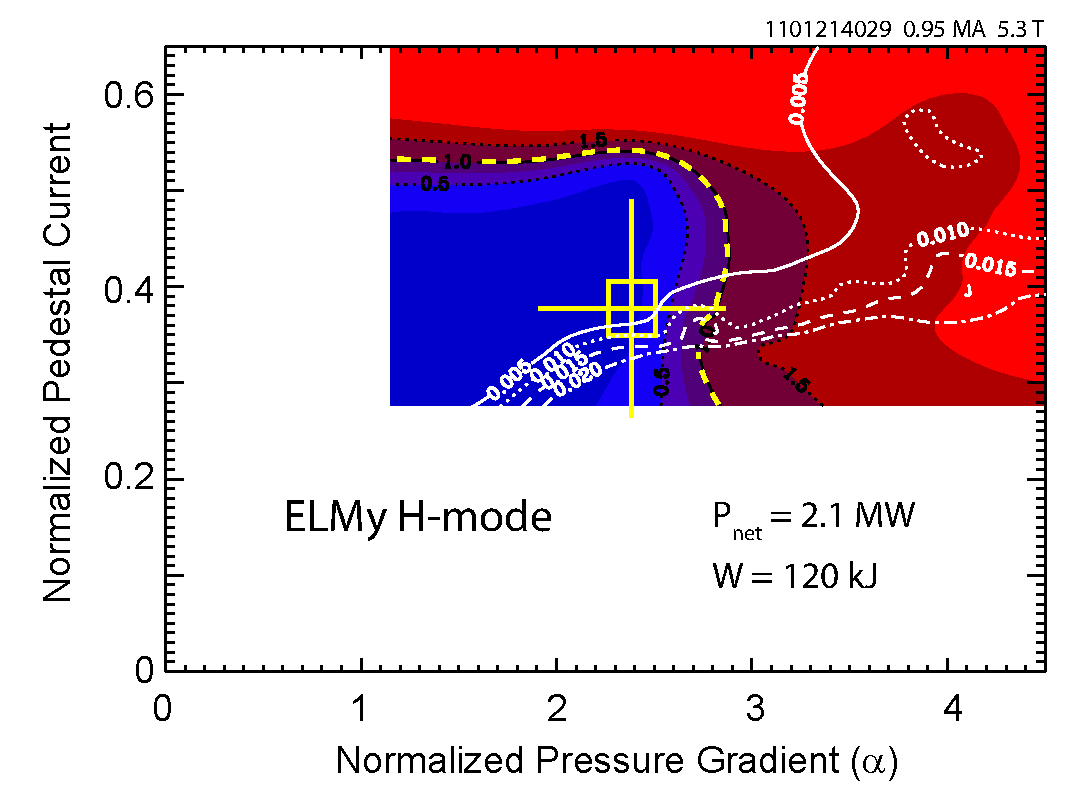
\includegraphics[width=0.8\textwidth]{graphics/ELMy/elmy_elite.pdf}

\end{frame}

%%%%%%%%%%%%%%%%%%%%%%%%%%%%%%%%%%%%%%%%%%%%%%%%%%%%%%%%%%%%%%%%%%%%%

\begin{frame}{EPED predicts pedestal height for ELM-binned pedestals}

\begin{columns}[c]
 \column{0.5\textwidth}
  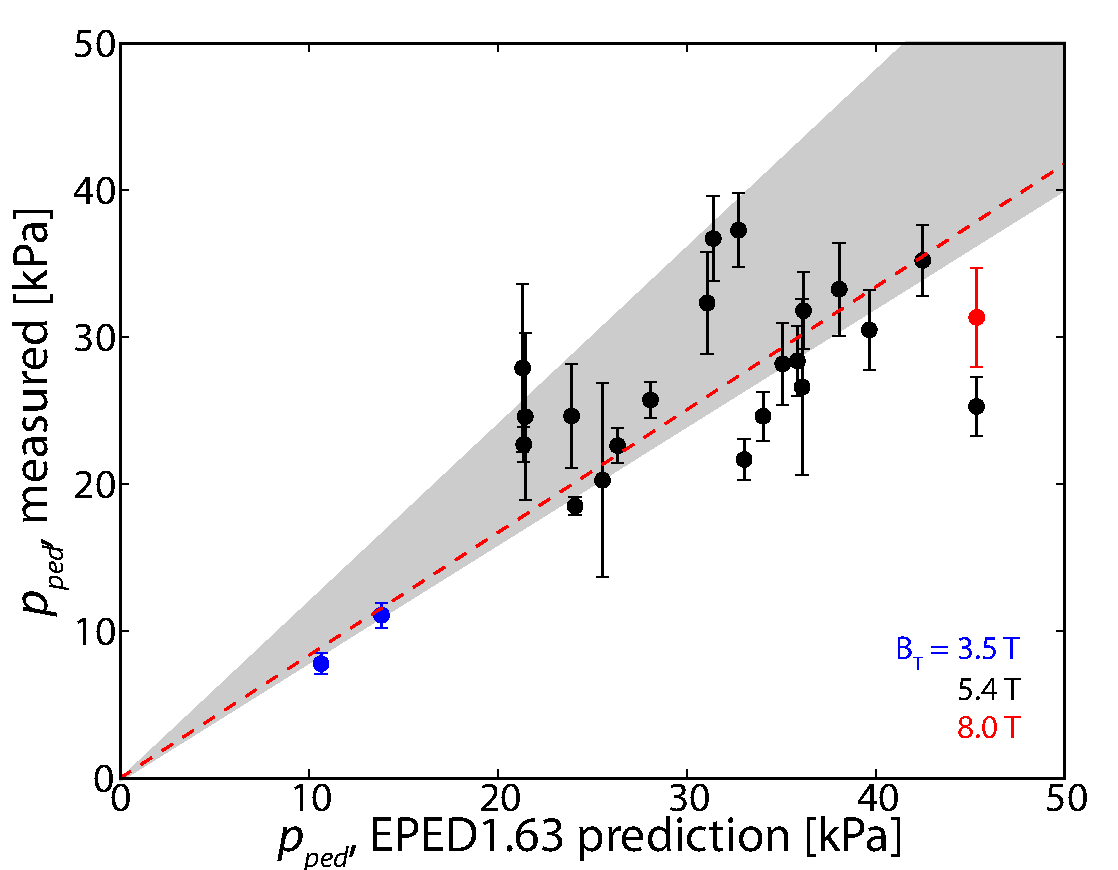
\includegraphics[width=\columnwidth]{graphics/ELMy/pped_EPED_meas.pdf}
 \column{0.5\textwidth}
  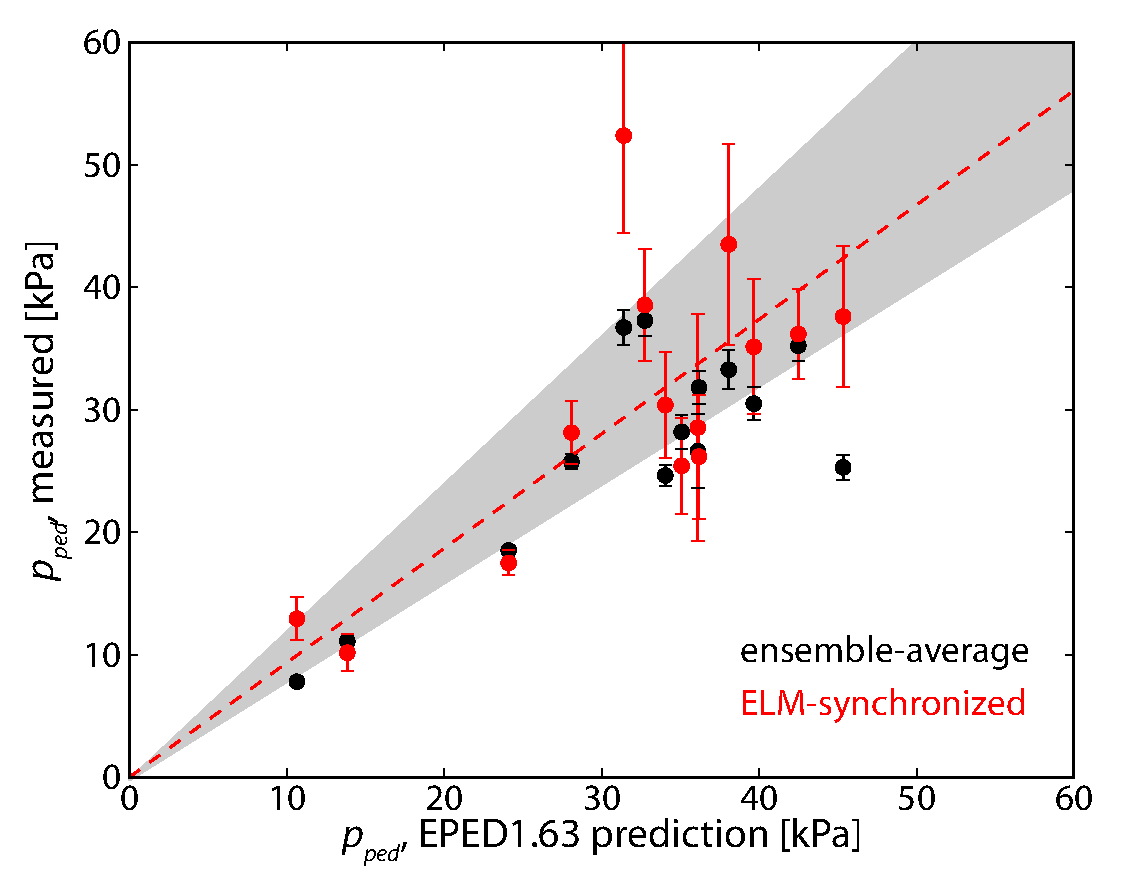
\includegraphics[width=\columnwidth]{graphics/ELMy/pped_EPED_elmsync.pdf}
\end{columns}

\large
\vspace{0.5em}
measured to predicted ratio of $0.835 \pm 0.036$ for ensemble-averaged data, $0.934 \pm 0.066$ for ELM-synced pedestals, well within expected $\pm 20\%$ accuracy for EPED predictions

\end{frame}

%%%%%%%%%%%%%%%%%%%%%%%%%%%%%%%%%%%%%%%%%%%%%%%%%%%%%%%%%%%%%%%%%%%%%

\begin{frame}{Width varies over narrow range, hard to predict}

\begin{columns}[c]
 \column{0.5\textwidth}
  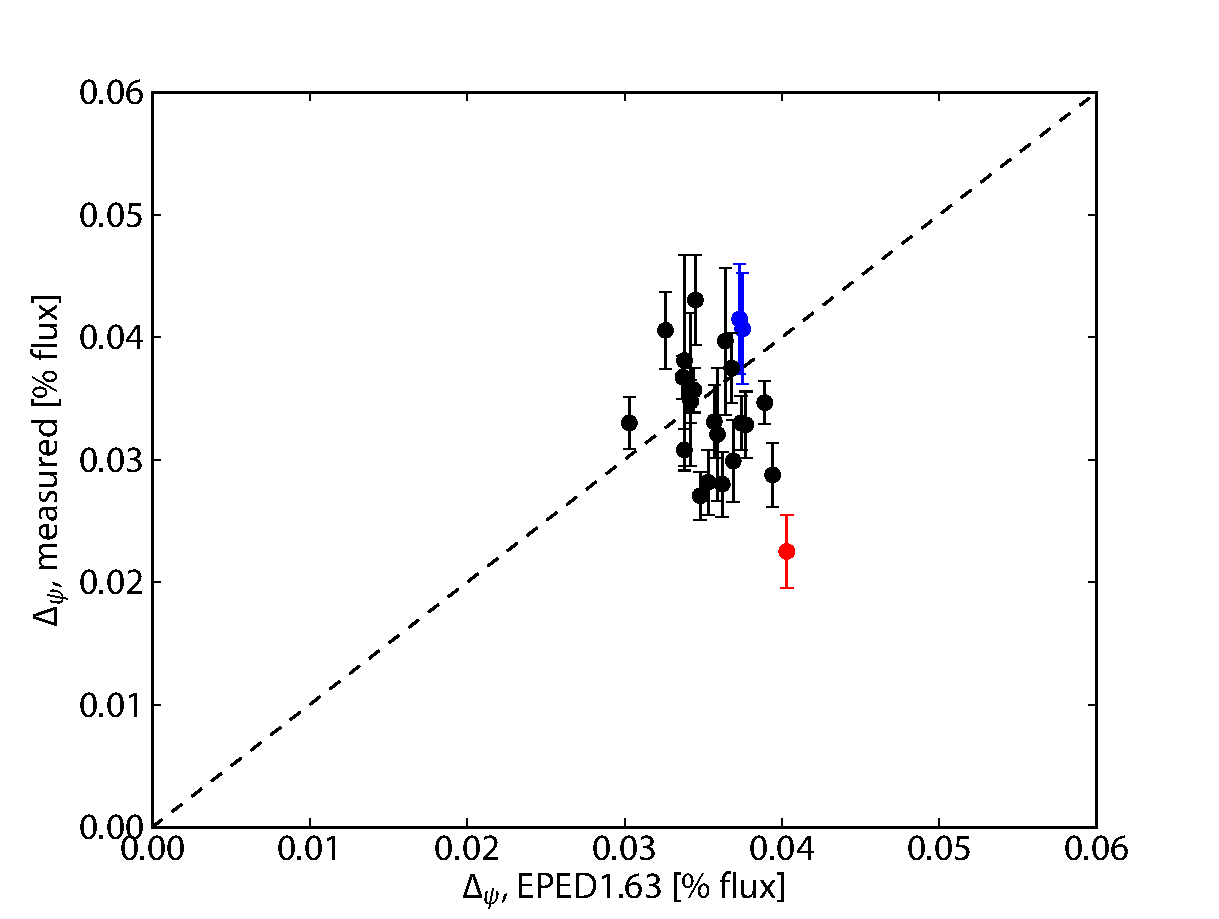
\includegraphics[width=\columnwidth]{graphics/ELMy/deltapsi_EPED_meas.pdf}
 \column{0.5\textwidth}
  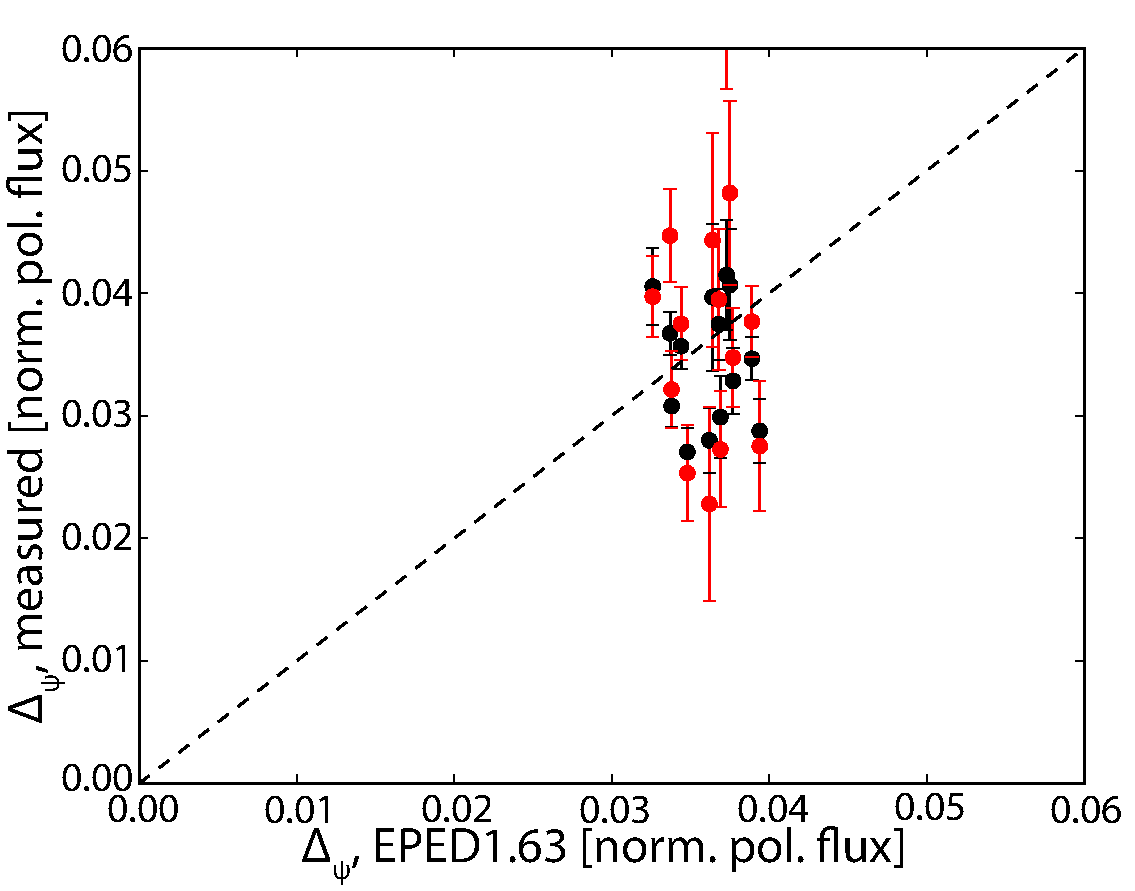
\includegraphics[width=\columnwidth]{graphics/ELMy/deltapsi_EPED_elmsync.pdf}
\end{columns}

\large
\vspace{0.5em}
Pedestal width varies little over range of $3-5\%$ of poloidal flux, difficult to extract trend -- EPED reproduces robust width to within $\pm 20\%$ uncertainty

\end{frame}

%%%%%%%%%%%%%%%%%%%%%%%%%%%%%%%%%%%%%%%%%%%%%%%%%%%%%%%%%%%%%%%%%%%%%

\begin{frame}{Experiments expand parameter space tested in EPED\footnote[5]{RJ Groebner \emph{et al.}, \emph{Nuclear Fusion} \textbf{53} (2013)}}

\begin{columns}[c]
 \column{0.5\textwidth}
  \begin{itemize}
   \large
   \item reach highest field ($\SI{8}{\tesla}$), highest thermal pressure, within factor of $\sim 2$ of ITER pedestal target
   \vspace{0.5em}
   \item C-Mod contribution to multi-machine Joint Research Target
   \vspace{0.5em}
   \item reliable physics-based understanding of H-mode pedestal limits
  \end{itemize}
 \column{0.5\textwidth}
  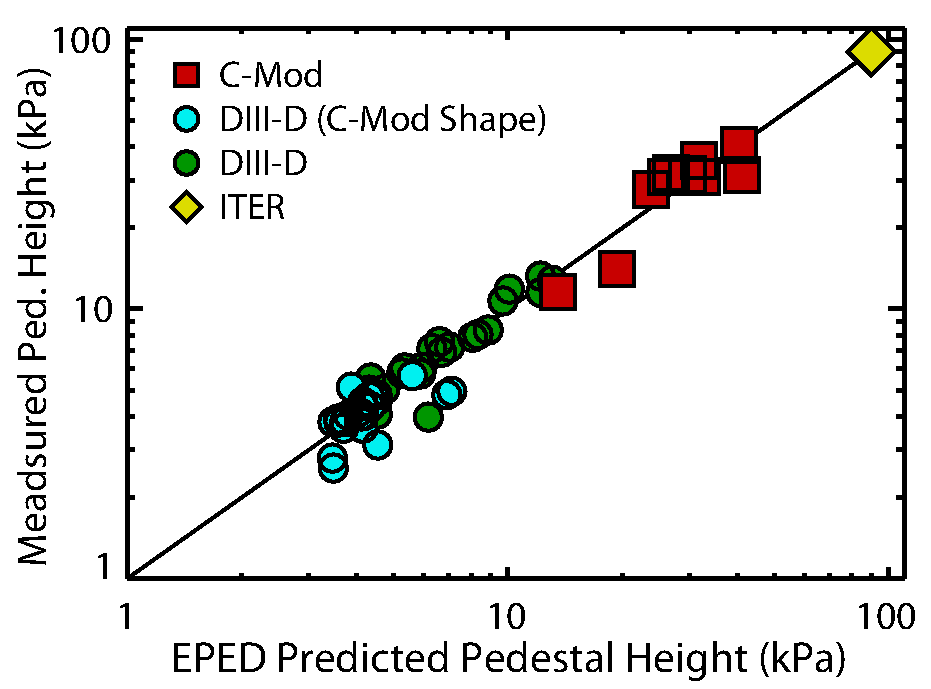
\includegraphics[width=\columnwidth]{graphics/ELMy/eped.pdf}
\end{columns}

\end{frame}

%%%%%%%%%%%%%%%%%%%%%%%%%%%%%%%%%%%%%%%%%%%%%%%%%%%%%%%%%%%%%%%%%%%%%

\begin{frame}{Outline}

 \setbeamercolor{normal text}{fg=gray,bg=}
 \setbeamercolor{alerted text}{fg=black,bg=}
 \usebeamercolor{normal text}

\begin{itemize}
 \large
 \alert<+>{\item \textbf{I-Mode Pedestals \& Global Performance}\footnote[2]{JR Walk \emph{et al.}, \emph{Physics of Plasmas} \textbf{21} (2014)}$^,$\footnote[3]{\emph{Invited talk}, APS-DPP Nov. 2013}
 \begin{itemize}
  \large
  \item Pedestal response to fueling, heating power
  \item Pedestal widths and gradients
  \item Global performance and confinement scalings
 \end{itemize}}
 \vspace{0.5em}
 \item \textbf{I-Mode Pedestal Stability}
 \begin{itemize}
  \large
  \item P-B MHD, KBM modeling
  \item ELM characterization
 \end{itemize}
 \vspace{0.5em}
 \item \textbf{Summary, Future Work, \& Questions}
\end{itemize}

\end{frame}

%%%%%%%%%%%%%%%%%%%%%%%%%%%%%%%%%%%%%%%%%%%%%%%%%%%%%%%%%%%%%%%%%%%%%

\begin{frame}{Temperature pedestal H-mode-like,\\ set by plasma current, heating power}

 \begin{columns}[c]
  \column{0.5\textwidth}
   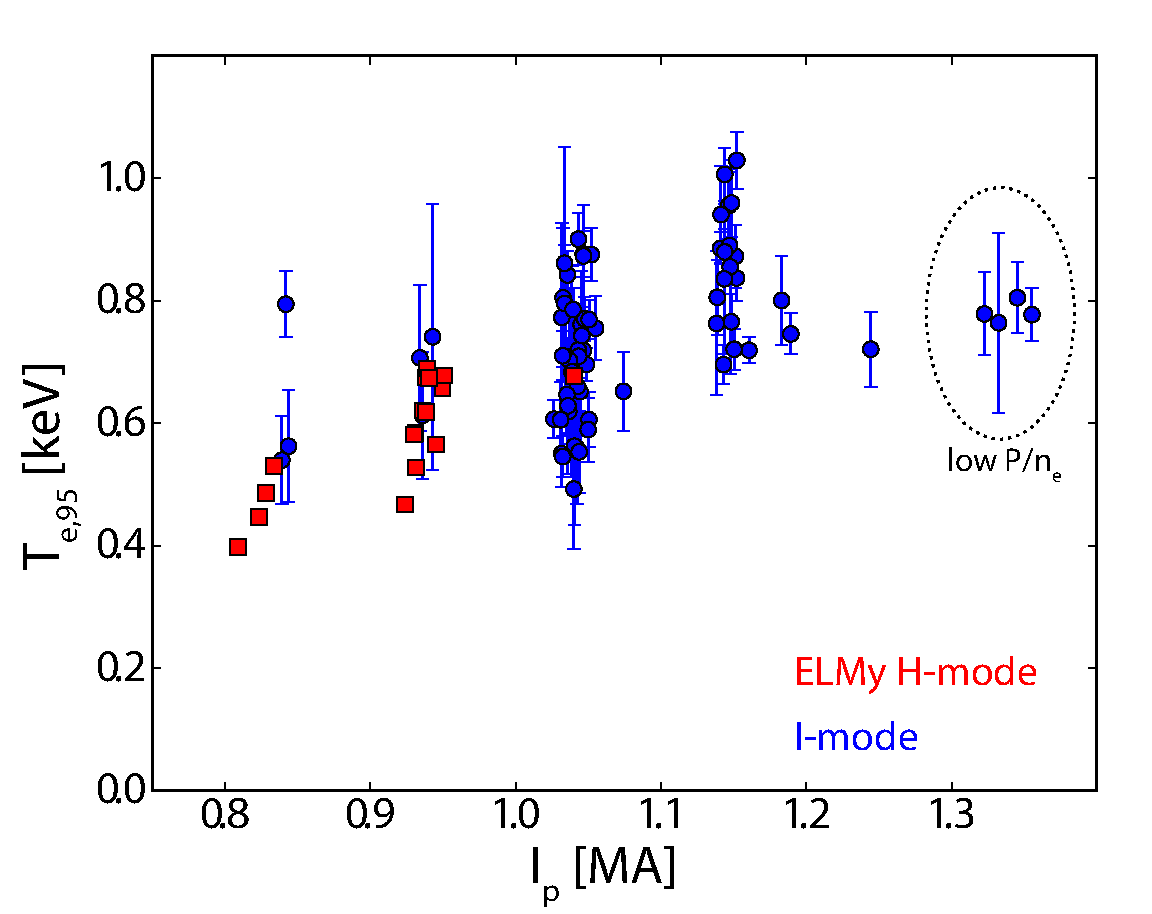
\includegraphics[width=\columnwidth]{graphics/IModePedestal/Ip_Te95.pdf}
  \column{0.5\textwidth}
   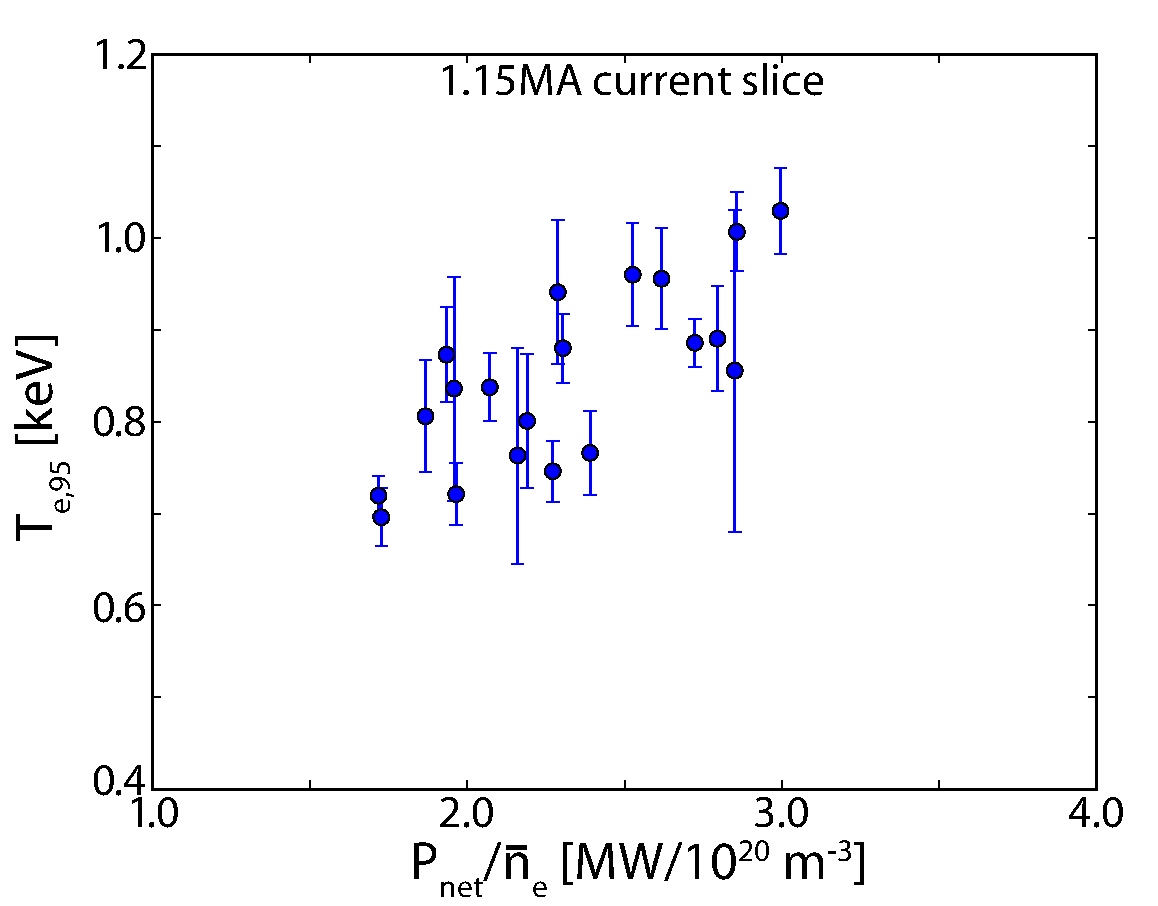
\includegraphics[width=\columnwidth]{graphics/IModePedestal/Pnebar_Te95_115MA.pdf}
 \end{columns}
 
 \vspace{0.5em}
 \begin{itemize}
  \item pedestal $T_e$ shows positive trending $T_e \sim I_p$, spread at given current due to heating power
  \item input power strongly affects pedestal temperature as with EDA H-mode -- more properly, \textcolor{red}{power per particle sets pedestal temperature} at fixed current
 \end{itemize}

\end{frame}

%%%%%%%%%%%%%%%%%%%%%%%%%%%%%%%%%%%%%%%%%%%%%%%%%%%%%%%%%%%%%%%%%%%%%

\begin{frame}{In contrast, density set by operator fueling,\\ with L-mode-like profile}

 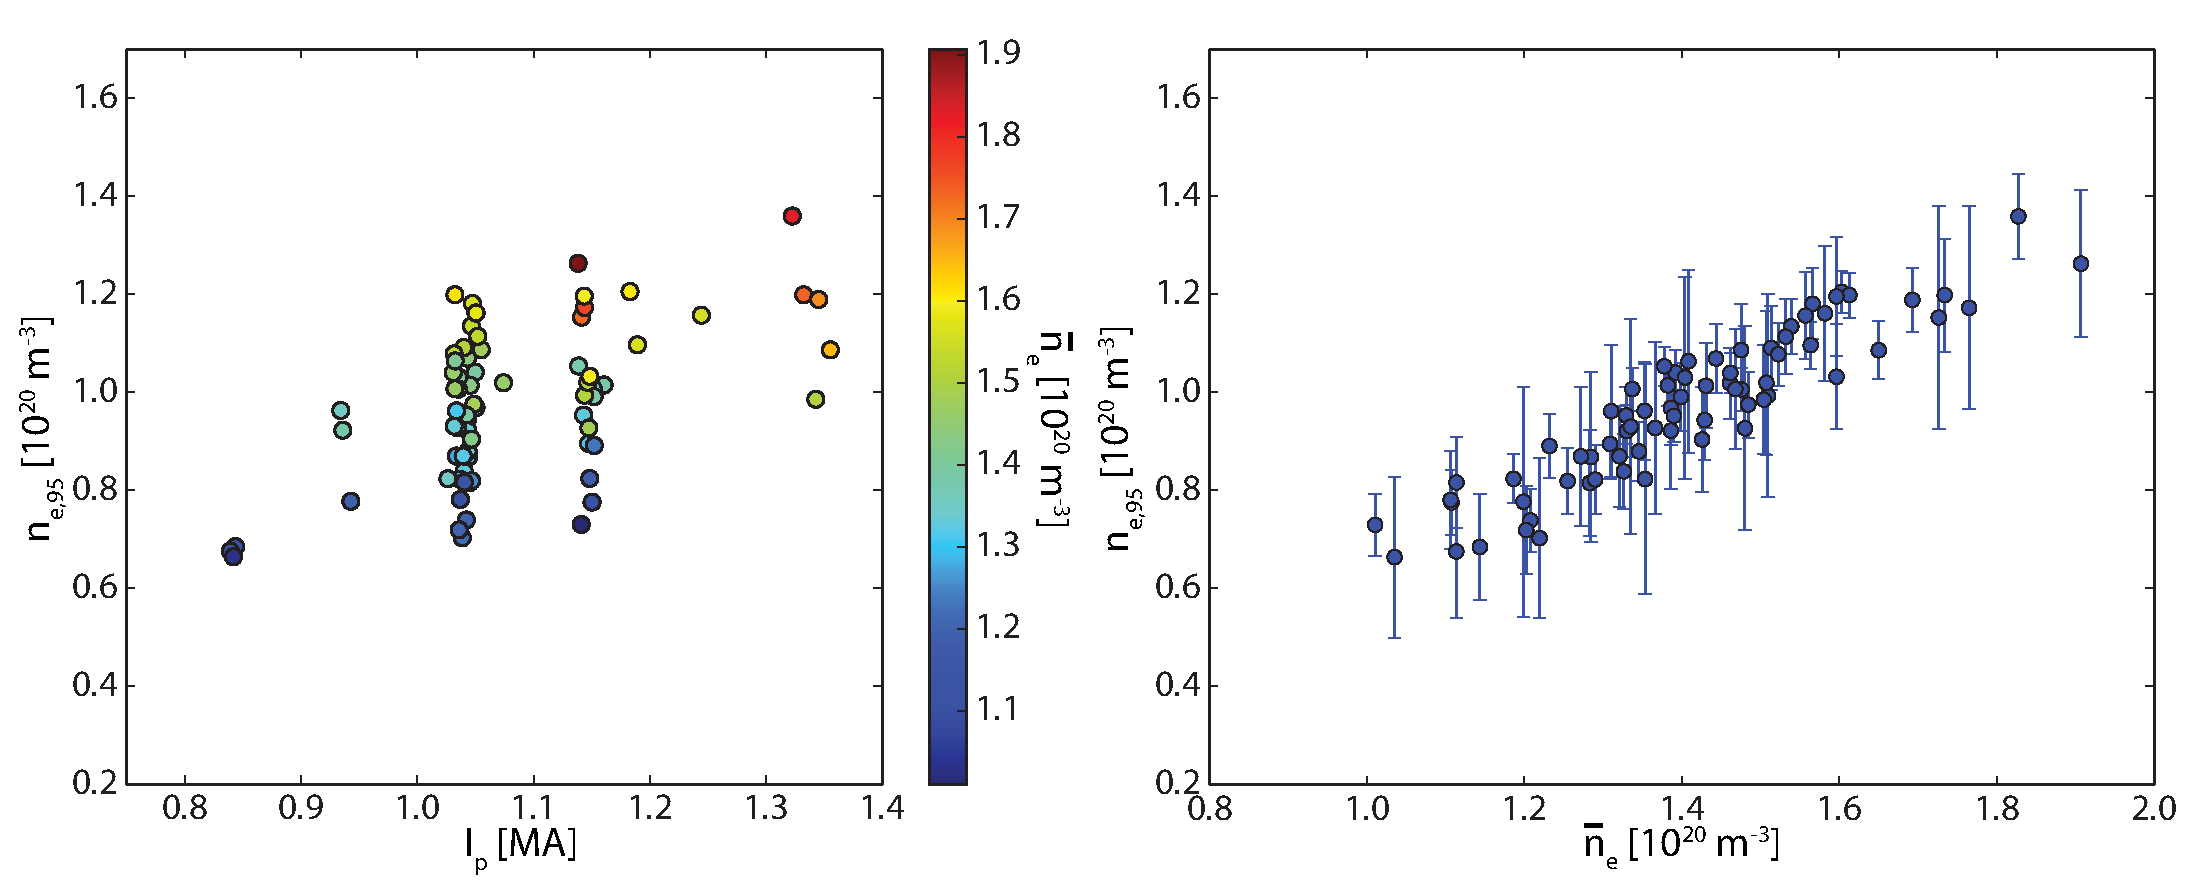
\includegraphics[width=\textwidth]{graphics/IModePedestal/imode_density.pdf}

\end{frame}

%%%%%%%%%%%%%%%%%%%%%%%%%%%%%%%%%%%%%%%%%%%%%%%%%%%%%%%%%%%%%%%%%%%%%

\begin{frame}{Pedestal density separately controlled from temperature, independent of MHD limits}

 \begin{columns}[c]
  \column{0.6\textwidth}
   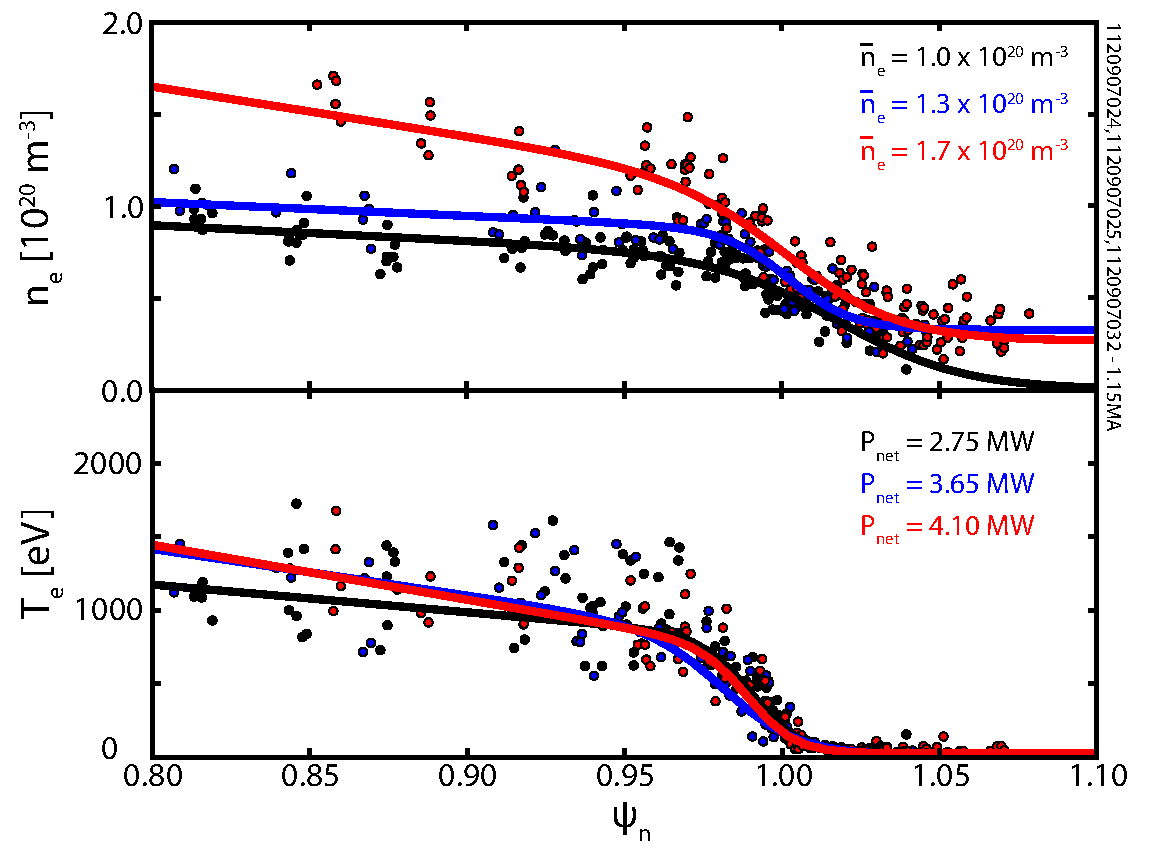
\includegraphics[width=\columnwidth]{graphics/IModePedestal/fuelingprofiles.pdf}
  \column{0.4\textwidth}
   \begin{itemize}
    \item with sufficient power to maintain $P_{net}/\overline{n}_e$, temperature pedestal matched across range of fueling
    \vspace{0.5em}
    \item Contrasts to MHD-limited pedestals (fixed $\beta_{p,ped} \rightarrow $ limit on $n_e T_e$) -- path to strongly increase pedestal beta
   \end{itemize}
 \end{columns}

\end{frame}

%%%%%%%%%%%%%%%%%%%%%%%%%%%%%%%%%%%%%%%%%%%%%%%%%%%%%%%%%%%%%%%%%%%%%

\begin{frame}{I-mode pedestal pressure scales with current, heating power, fueling, competitive to H-mode}

 \begin{columns}[c]
  \column{0.5\textwidth}
   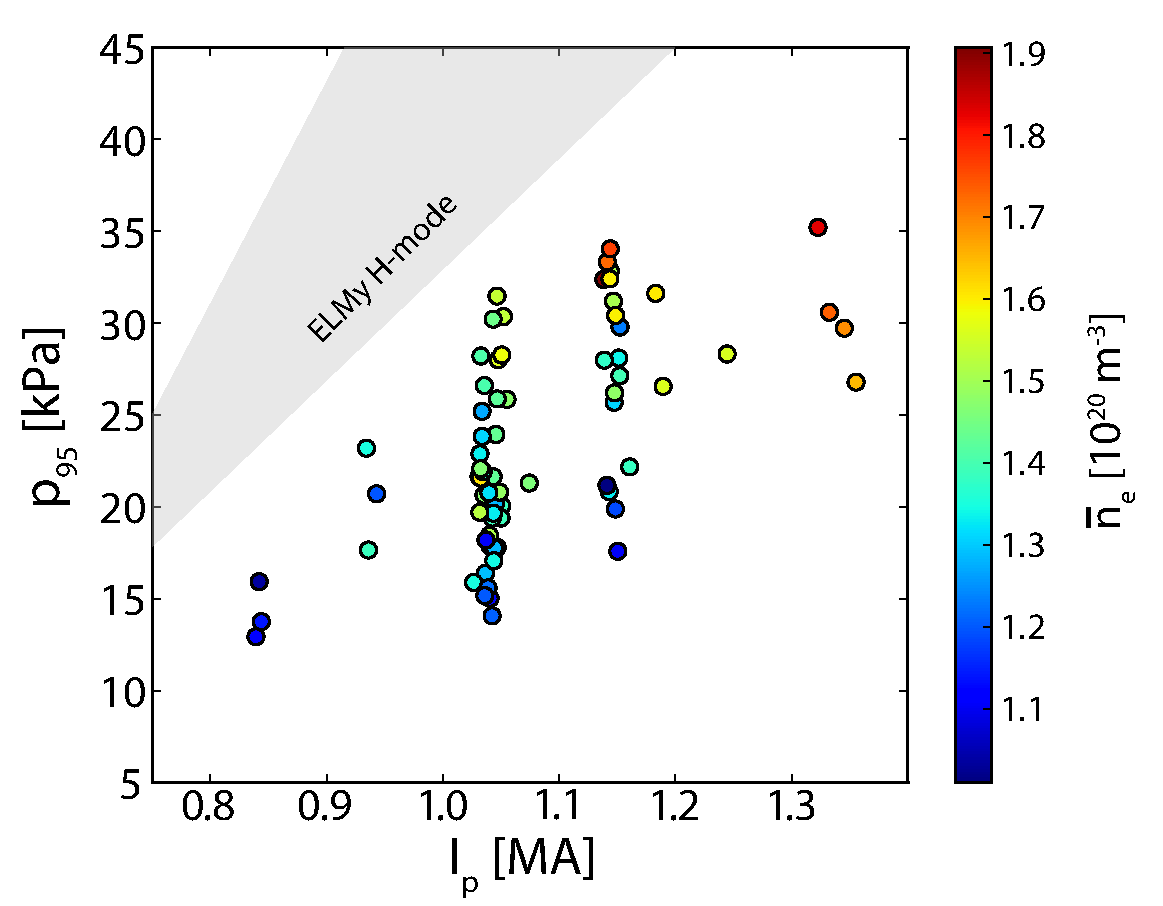
\includegraphics[width=\columnwidth]{graphics/IModePedestal/Ip_p95_nebar.pdf}
  \column{0.5\textwidth}
   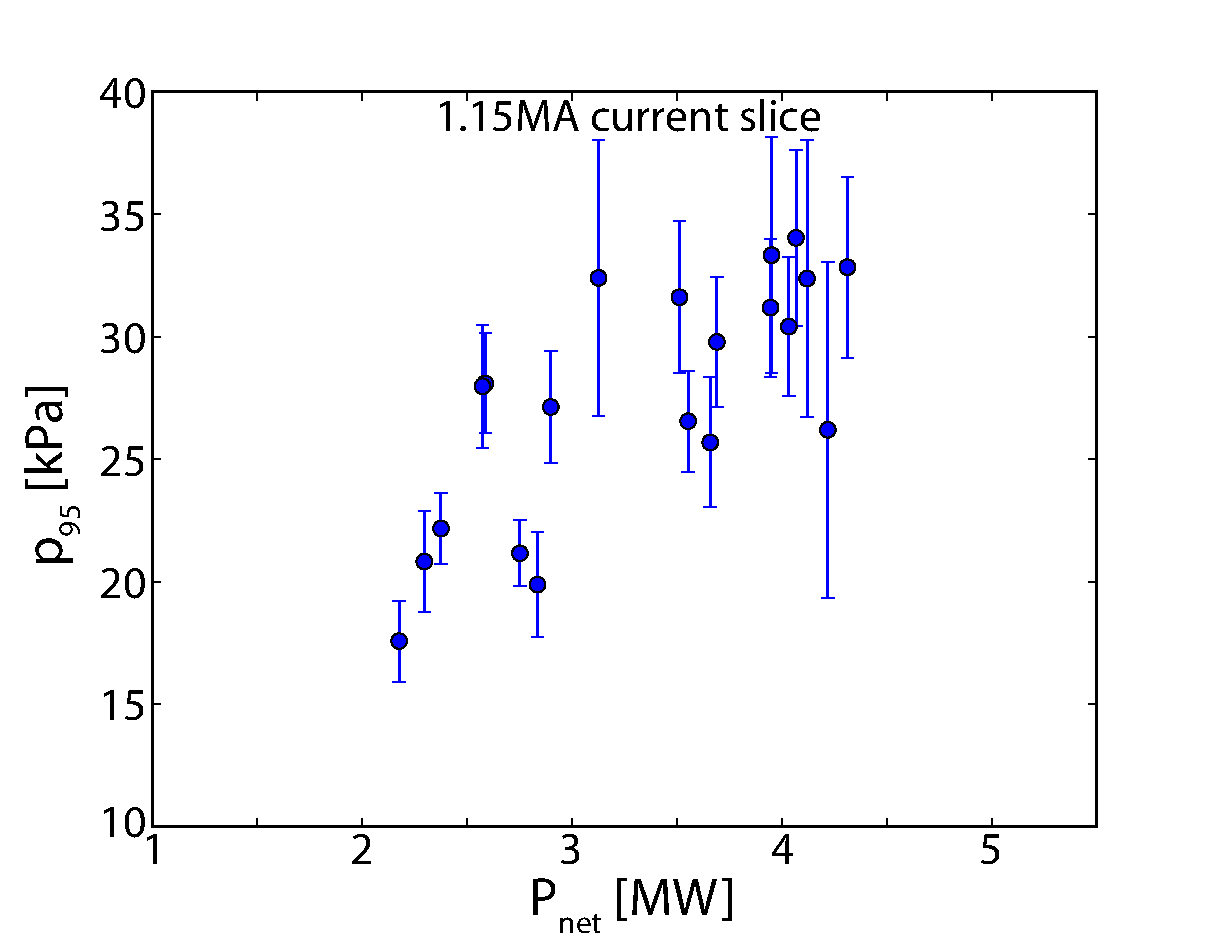
\includegraphics[width=\columnwidth]{graphics/IModePedestal/Pnet_p95_115MA.pdf}
 \end{columns}
 
  \begin{itemize}
  \item Pedestal pressure increases at least as $p_{ped} \sim I_p$, due to increased $T_e \sim I_p$ and more fueling (fixed $f_{Gr}$) at higher current
  \item Pedestal pressure at fixed current $\sim P_{net}$ (consistent with $T_e \sim P/n_e$), corresponds to favorable scaling of energy confinement with heating power
  \item Fueling (with sufficient power to maintain temperature pedestal) strongly increases pedestal pressure
 \end{itemize}

\end{frame}

%%%%%%%%%%%%%%%%%%%%%%%%%%%%%%%%%%%%%%%%%%%%%%%%%%%%%%%%%%%%%%%%%%%%%

\begin{frame}{What does this get us?}

 

\end{frame}

%%%%%%%%%%%%%%%%%%%%%%%%%%%%%%%%%%%%%%%%%%%%%%%%%%%%%%%%%%%%%%%%%%%%%

\begin{frame}{Pedestal impacts core, global performance}

 \centering
 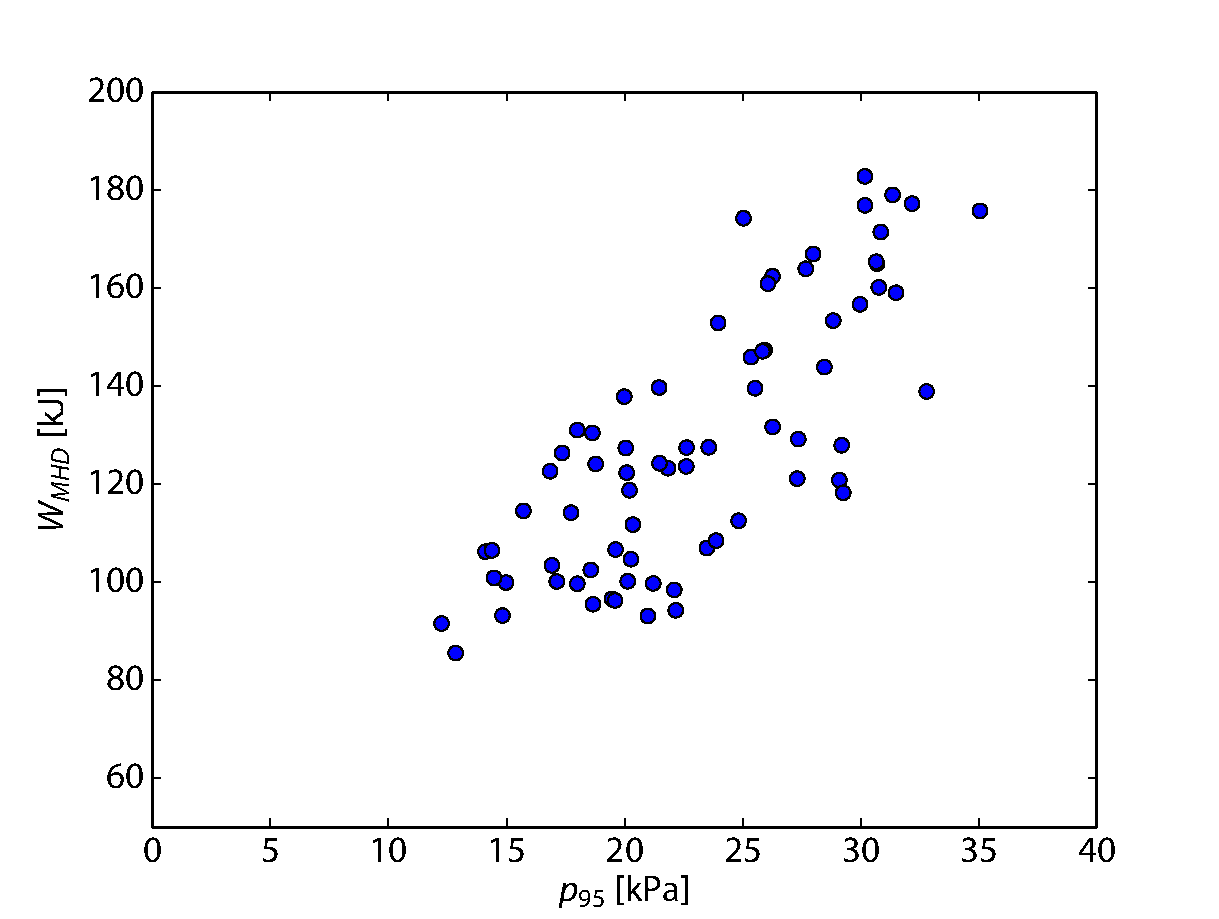
\includegraphics[width=0.8\textwidth]{graphics/IModePedestal/p95_W.pdf}

\end{frame}

%%%%%%%%%%%%%%%%%%%%%%%%%%%%%%%%%%%%%%%%%%%%%%%%%%%%%%%%%%%%%%%%%%%%%

\begin{frame}{Strong temperature pedestal supports high\\ core temperature, pressure}

 \begin{columns}[c]
  \column{0.45\textwidth}
   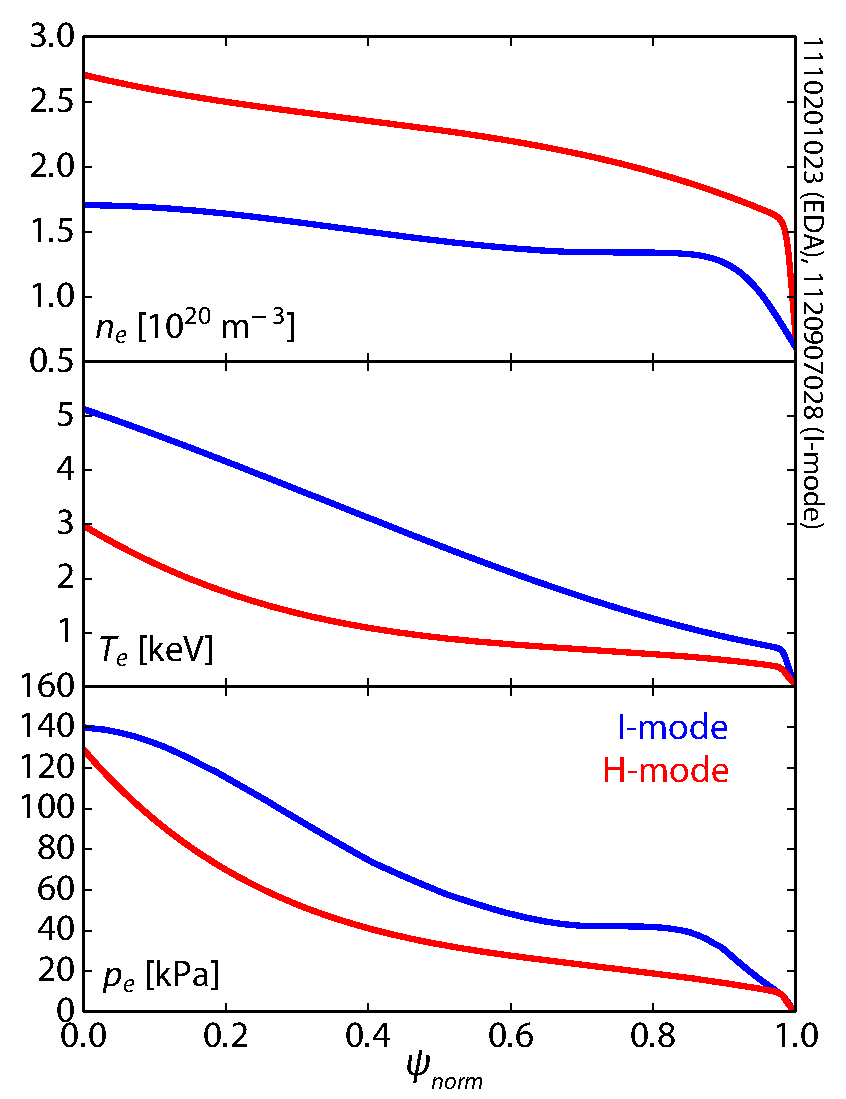
\includegraphics[width=\columnwidth]{graphics/IModePedestal/coreprof_v2.pdf}
  \only<1>{\column{0.55\textwidth}
   \begin{itemize}
    \large
    \item stiff ($R/L_{T_e} \sim$ fixed) temperature profiles $\rightarrow$ higher $T_{ped}$ supports greatly increased core temperatures
    \item provided moderated density peaking ($n_{e,0}/\langle n_e \rangle \sim 1.1-1.3$ in I-mode), reaches comparable core, vol-average pressure despite relaxed $p_{ped}$
    \item fusion-reactive plasma where $T_e > \SI{4}{\kilo\electronvolt}$, high $T_{ped}$ maximizes fusing volume
   \end{itemize}}
   \only<2>{\column{0.55\textwidth}
   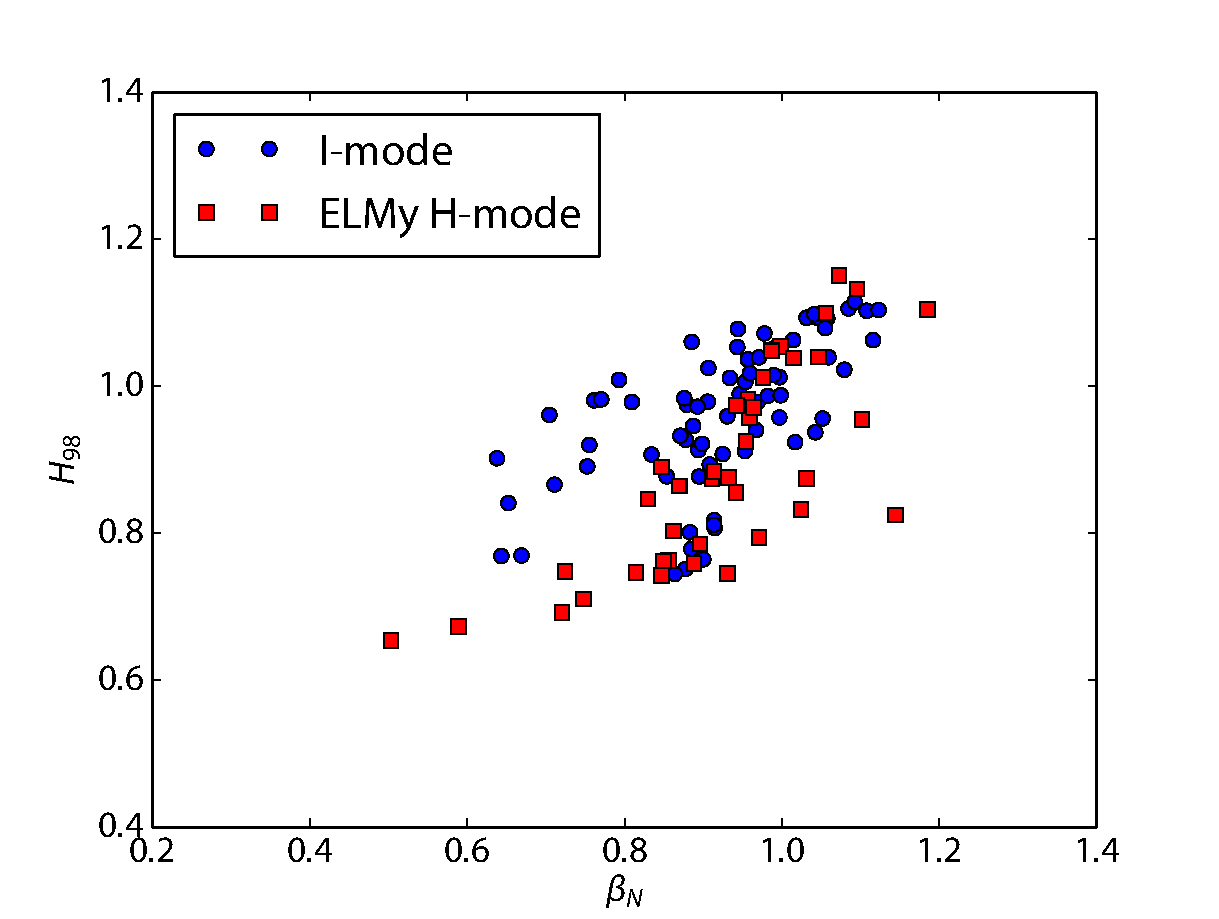
\includegraphics[width=\columnwidth]{graphics/IModePedestal/betan_H_i_e.pdf}
   
   \large
   $\rightarrow$ same $\langle \beta_N \rangle$, normalized confinement to ELMy H-mode   
   }
 \end{columns}

\end{frame}

%%%%%%%%%%%%%%%%%%%%%%%%%%%%%%%%%%%%%%%%%%%%%%%%%%%%%%%%%%%%%%%%%%%%%

\begin{frame}{Energy confinement lacks degradation with heating power}

 \begin{columns}[c]
  \column{0.5\textwidth}
   \begin{itemize}
    \large
    \item Stored energy $W \sim P \tau_E$
    \vspace{0.5em}
    \item for H-mode, expect $\tau_E \sim I_p$, with power degradation $\tau_E \sim P^{-0.7}$ thus $W \sim I_p P^{0.3}$
    \vspace{0.5em}
    \item I-mode stored energy $W \sim I_p P_{net} \rightarrow$ little/no degradation of $\tau_E$ with heating power
    \vspace{0.5em}
    \item reflects lack of MHD limit on pedestal
   \end{itemize}
  \column{0.5\textwidth}
   \centering
   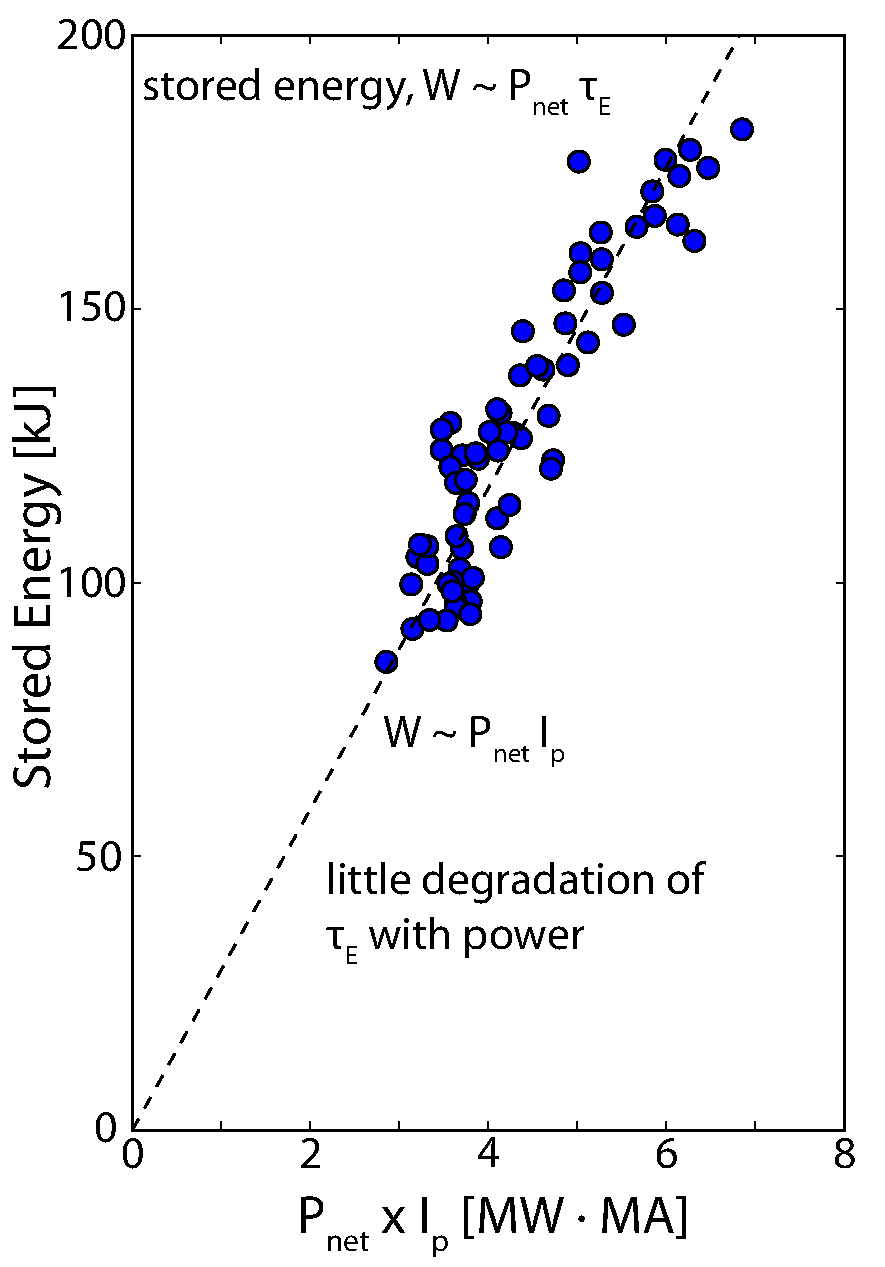
\includegraphics[width=0.85\columnwidth]{graphics/IModePedestal/PIp_W_scale.pdf}
 \end{columns}

\end{frame}

%%%%%%%%%%%%%%%%%%%%%%%%%%%%%%%%%%%%%%%%%%%%%%%%%%%%%%%%%%%%%%%%%%%%%

\begin{frame}{...As well as with fueling}

 \begin{columns}[c]
  \column{0.6\textwidth}
   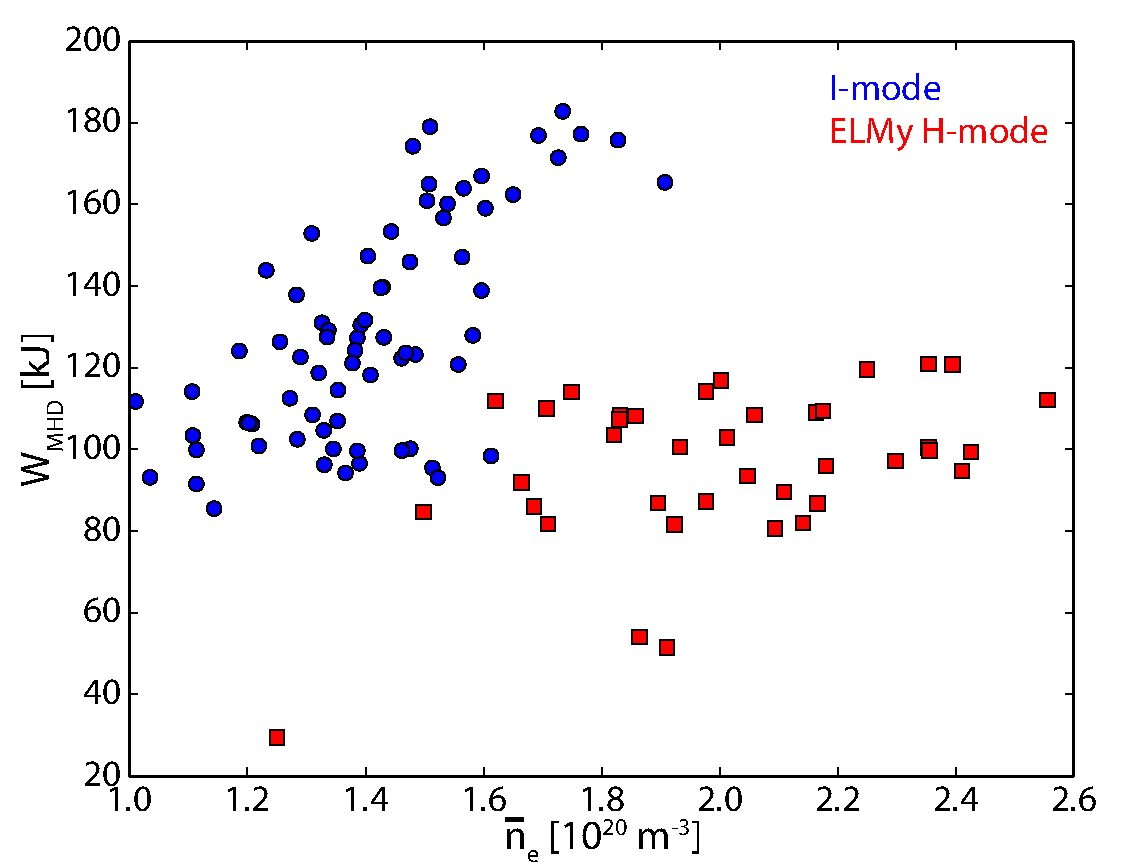
\includegraphics[width=\columnwidth]{graphics/IModePedestal/nebar_W_i_e.pdf}
  \column{0.4\textwidth}
   \begin{itemize}
    \large
    \item I-mode stored energy set by pedestal pressure, responding strongly to fueling
    \vspace{0.5em}
    \item ELMy H-mode stored energy set by pedestal $\beta_p$, limited by MHD constraint -- mainly increase pedestal $\beta_p$ with stronger shaping, flat relation with fueling
   \end{itemize}
 \end{columns}

\end{frame}

%%%%%%%%%%%%%%%%%%%%%%%%%%%%%%%%%%%%%%%%%%%%%%%%%%%%%%%%%%%%%%%%%%%%%

\begin{frame}{}

 how much detail for confinement scalings?

\end{frame}

%%%%%%%%%%%%%%%%%%%%%%%%%%%%%%%%%%%%%%%%%%%%%%%%%%%%%%%%%%%%%%%%%%%%%

\begin{frame}{Outline}

 \setbeamercolor{normal text}{fg=gray,bg=}
 \setbeamercolor{alerted text}{fg=black,bg=}
 \usebeamercolor{normal text}

\begin{itemize}
 \large
 \item \textbf{I-Mode Pedestals \& Global Performance}\footnote[2]{JR Walk \emph{et al.}, \emph{Physics of Plasmas} \textbf{21} (2014)}$^,$\footnote[3]{\emph{Invited talk}, APS-DPP Nov. 2013}
 \begin{itemize}
  \large
  \item Pedestal response to fueling, heating power
  \item Pedestal widths and gradients
  \item Global performance and confinement scalings
 \end{itemize}
 \vspace{0.5em}
 \alert<+>{\item \textbf{I-Mode Pedestal Stability}
 \begin{itemize}
  \large
  \item P-B MHD, KBM modeling
  \item ELM characterization
 \end{itemize}}
 \vspace{0.5em}
 \item \textbf{Summary, Future Work, \& Questions}
\end{itemize}

\end{frame}

%%%%%%%%%%%%%%%%%%%%%%%%%%%%%%%%%%%%%%%%%%%%%%%%%%%%%%%%%%%%%%%%%%%%%

\begin{frame}{Pedestal pressure gradient suggests MHD stability, headroom for performance improvement}

 \begin{columns}[c]
  \column{0.6\textwidth}
   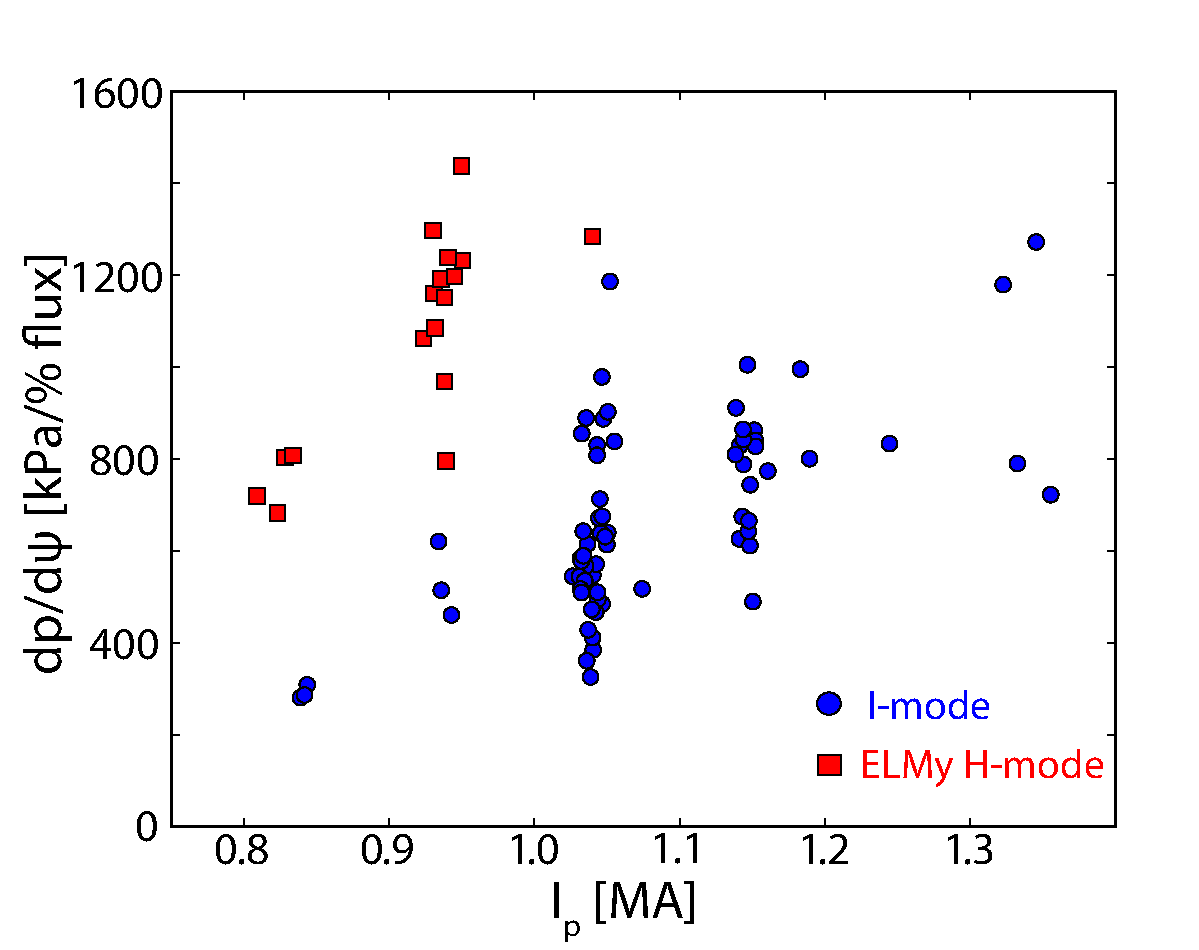
\includegraphics[width=\columnwidth]{graphics/IModePedestal/Ip_gradp.pdf}
  \column{0.4\textwidth}
   \begin{itemize}
    \large
    \item Pedestal $\nabla p$ shallower at given $I_p$ than ELMy H-mode due to lack of density pedestal
    \vspace{0.5em}
    \item Gradients scale more weakly than $\nabla p \propto I_p^2$ from ballooning MHD (critical-gradient) stability boundary
   \end{itemize}
 \end{columns}

\end{frame}

%%%%%%%%%%%%%%%%%%%%%%%%%%%%%%%%%%%%%%%%%%%%%%%%%%%%%%%%%%%%%%%%%%%%%

\begin{frame}{I-mode pedestal scalings consistent with stability\\ against peeling-ballooning MHD}

 \setbeamercolor{normal text}{fg=gray,bg=}
 \setbeamercolor{alerted text}{fg=black,bg=}
 \usebeamercolor{normal text}

 \begin{columns}[c]
  \column{0.6\textwidth}
   \includegraphics<1>[width=\columnwidth]{graphics/IModeModeling/neBp_TeBp_elmy.pdf}
   \includegraphics<2>[width=\columnwidth]{graphics/IModeModeling/neBp_pBp.pdf}
  \column{0.4\textwidth}
   \begin{itemize}
    \large
    \alert<1>{\item ballooning stability, to lowest order, limits pedestal $\beta_p$ in ELMy H-mode; I-mode $n_e$, $T_e$ independent, rather than fixed $n_e T_e$}
    \vspace{0.5em}
    \alert<2>{\item Pedestal $\beta_p$ scaling with density consistent with constant $T_{e,95}/B_p \rightarrow T_e \sim I_p$, rather than $T_e \sim 1/n_e$}
   \end{itemize}
 \end{columns}

\end{frame}

%%%%%%%%%%%%%%%%%%%%%%%%%%%%%%%%%%%%%%%%%%%%%%%%%%%%%%%%%%%%%%%%%%%%%

\begin{frame}{Stability is self-enforcing for I-mode pedestals}

 \centering
 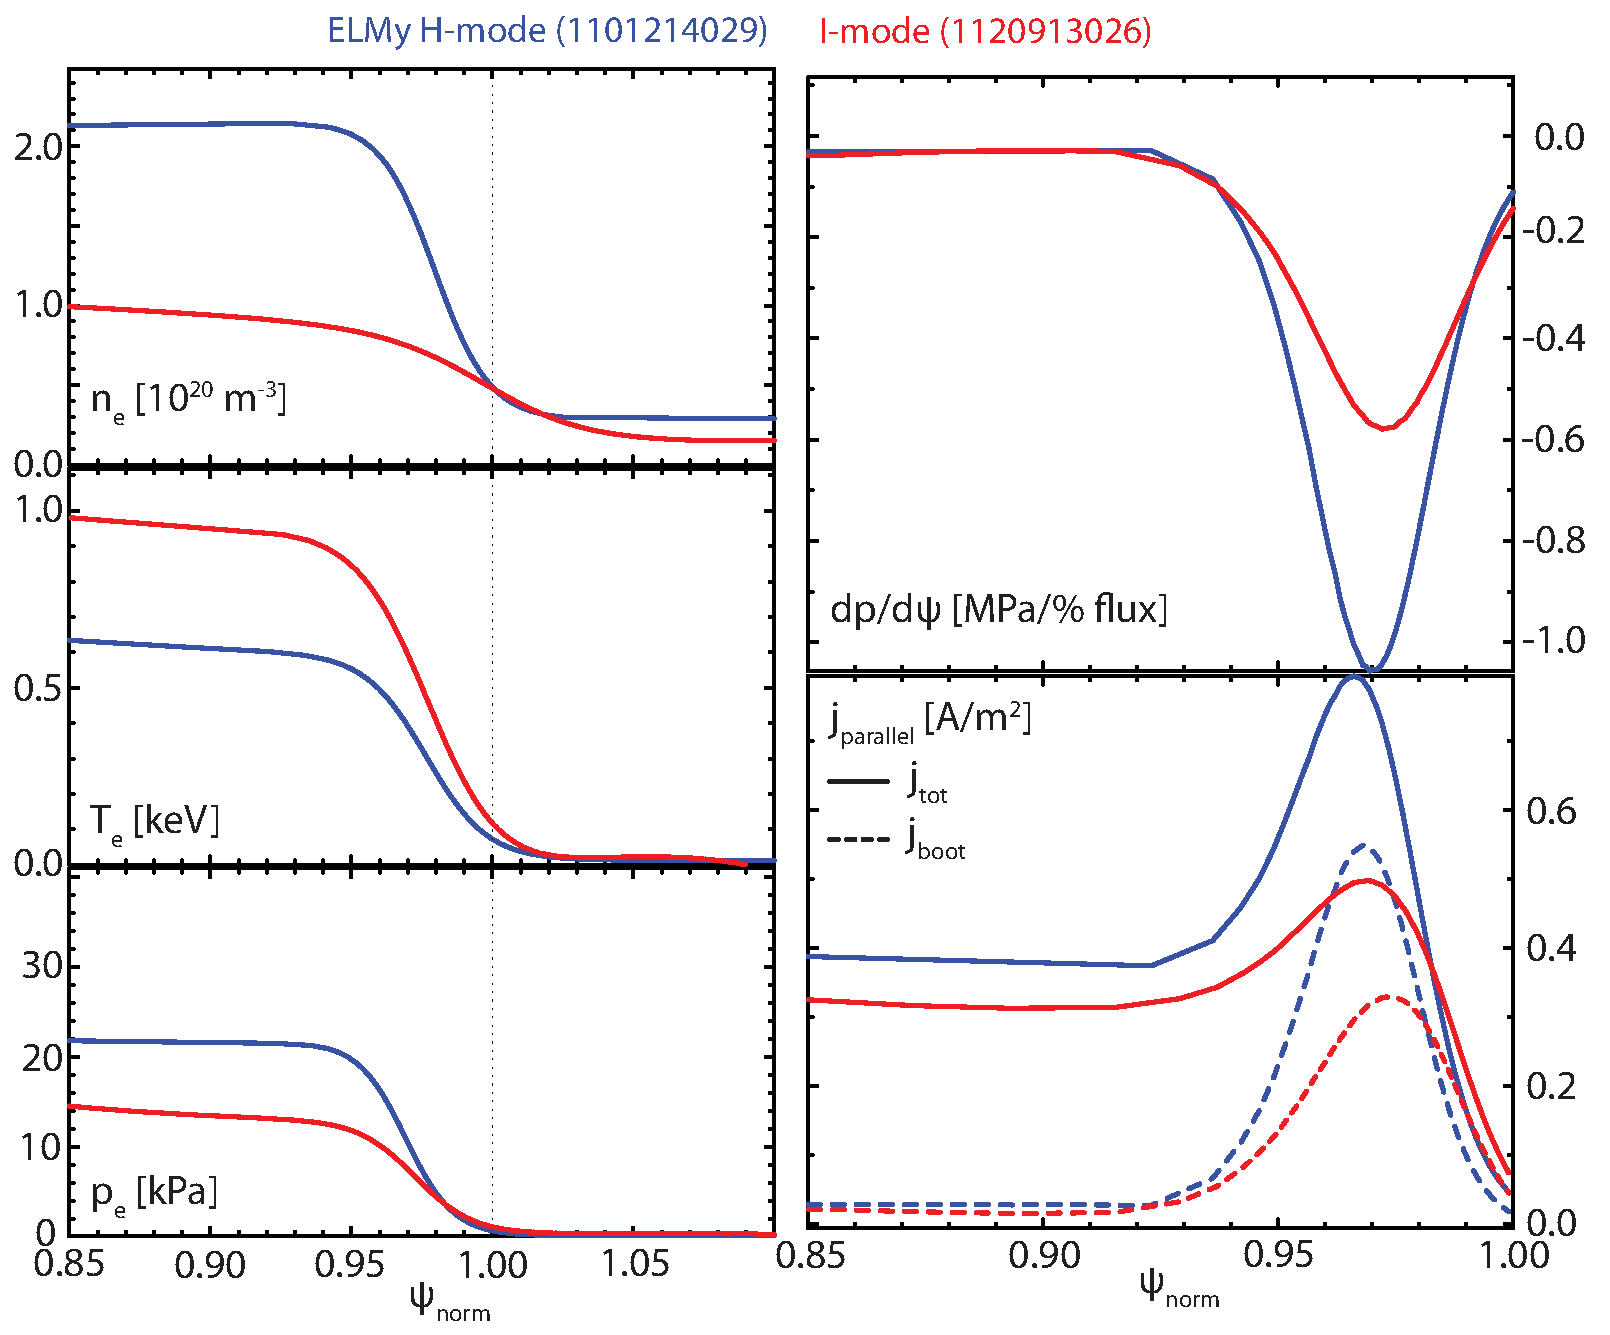
\includegraphics[width=0.8\textwidth]{graphics/IModeModeling/prof_elmy_imode.pdf}

\end{frame}

%%%%%%%%%%%%%%%%%%%%%%%%%%%%%%%%%%%%%%%%%%%%%%%%%%%%%%%%%%%%%%%%%%%%%

\begin{frame}{I-mode pedestal strongly stable against\\ peeling-ballooning MHD, KBM turbulence}

 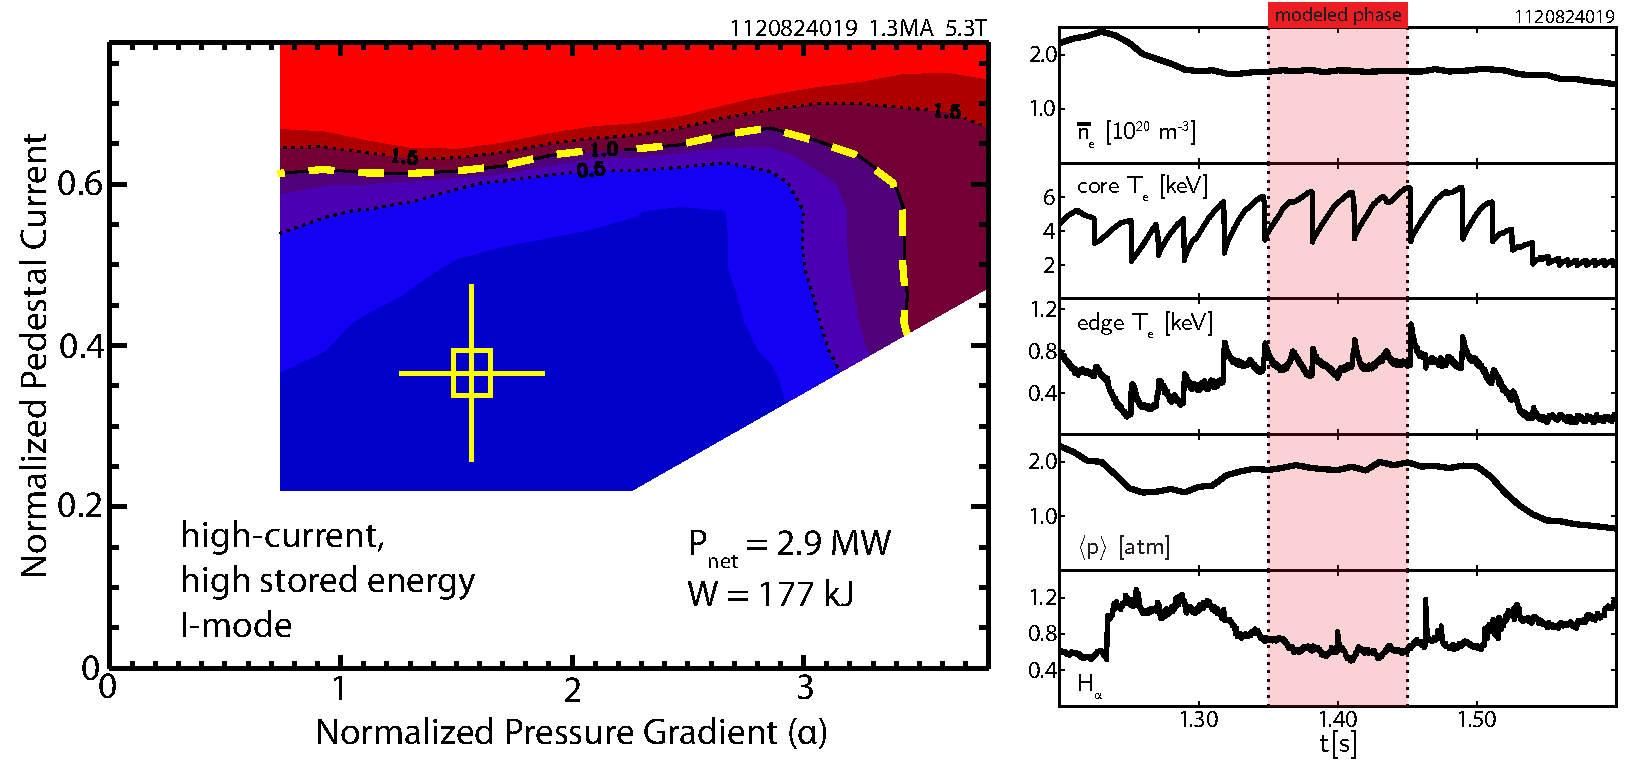
\includegraphics[width=\textwidth]{graphics/IModeModeling/1120824019_ELITE_stitch.pdf}

\end{frame}

%%%%%%%%%%%%%%%%%%%%%%%%%%%%%%%%%%%%%%%%%%%%%%%%%%%%%%%%%%%%%%%%%%%%%

\begin{frame}{Including in low-field, low-energy cases\\ exhibiting apparent ELMs}

 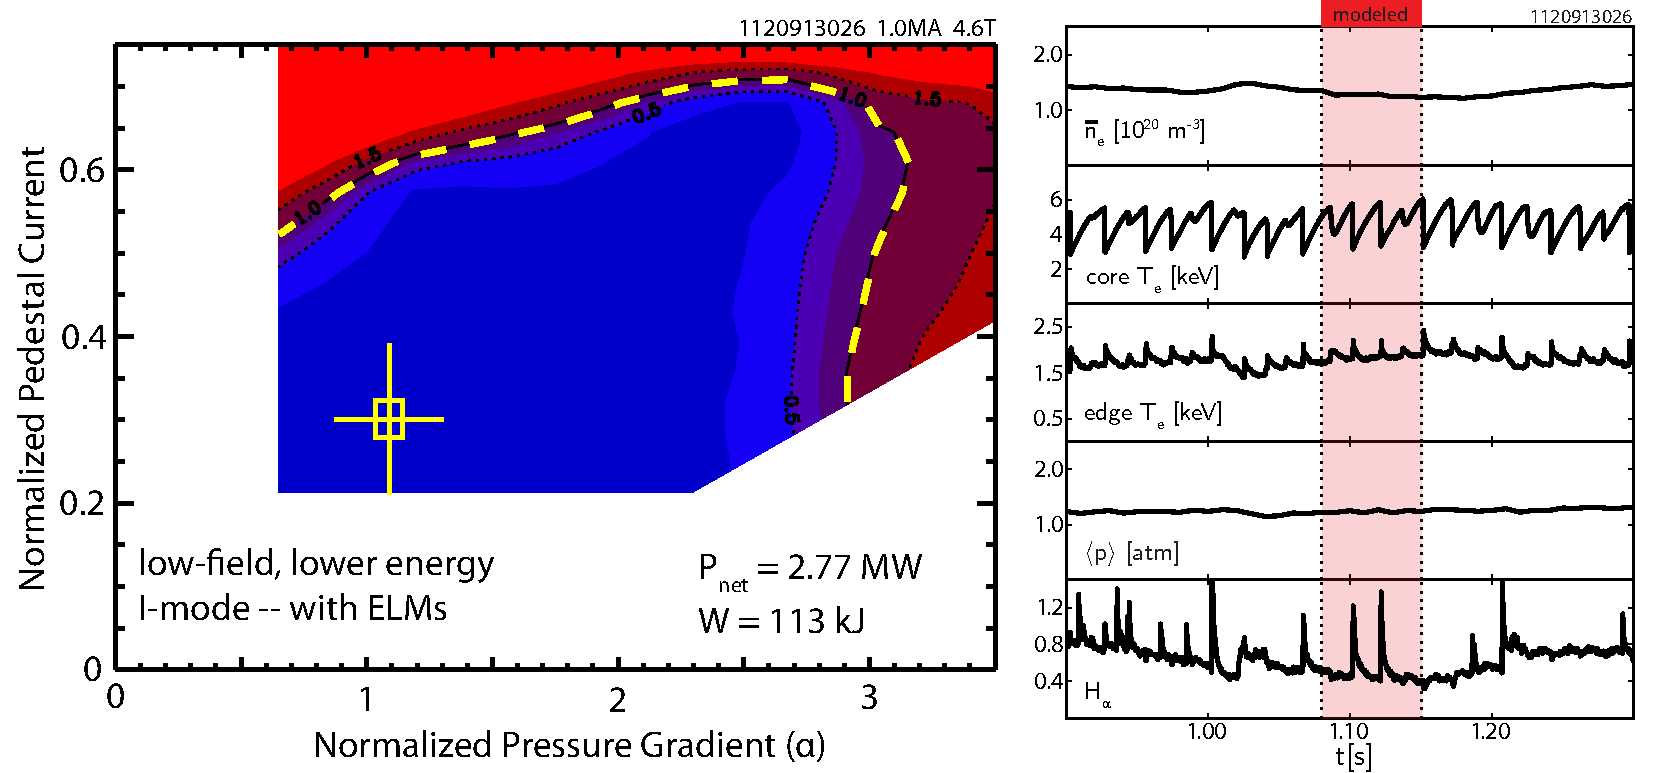
\includegraphics[width=\textwidth]{graphics/IModeModeling/1120913026_ELITE_stitch.pdf}

\end{frame}

%%%%%%%%%%%%%%%%%%%%%%%%%%%%%%%%%%%%%%%%%%%%%%%%%%%%%%%%%%%%%%%%%%%%%

\begin{frame}{I-mode pedestal modeled to be below KBM threshold\\ as well, including cases with ELMs}

 \begin{columns}[c]
  \column{0.6\textwidth}
   \includegraphics<1>[width=\columnwidth]{graphics/IModeModeling/1120824019_1400n5_35_gamws16_bal.pdf}
   \includegraphics<2>[width=\columnwidth]{graphics/IModeModeling/1120913026_1186n5_35_bal_jalpha.pdf}
  \column{0.4\textwidth}
   \begin{itemize}
    \large
    \item KBM-limited (EPED1) prediction for width, $\Delta_{EPED} = 0.076 \beta_{p,ped}^{1/2}$
    \vspace{0.5em}
    \item BALOO calculates width of pedestal locally beyond threshold -- mode onset when half of pedestal is unstable
    \vspace{0.5em}
    \item I-mode cases spanning width range modeled below threshold
   \end{itemize}
 \end{columns}

\end{frame}

%%%%%%%%%%%%%%%%%%%%%%%%%%%%%%%%%%%%%%%%%%%%%%%%%%%%%%%%%%%%%%%%%%%%%

\begin{frame}{EPED physics assumptions alone are not capturing all observed edge behavior in I-mode}

 \large
 I-mode pedestal is stable against identified ELM triggers -- however, in minority of cases (12 time windows / 10 unique shots, out of dataset of 72 time windows / 52 shots), particularly at low field ($\sim \SI{4.6}{\tesla}$) exhibit small, intermittent events that appear to be ELMs.
 
 \vspace{1em}
 $\rightarrow$ need to more carefully characterize these events!

\end{frame}

%%%%%%%%%%%%%%%%%%%%%%%%%%%%%%%%%%%%%%%%%%%%%%%%%%%%%%%%%%%%%%%%%%%%%

\begin{frame}{What is an ELM?}

 \large
 ELMs denoted by:
 \begin{itemize}
  \large
  \item burst of ionization in edge $\rightarrow$ spike in $H_\alpha$ light
  \item ``explosive'' crash in pedestal, both temperature and pressure
  \item unstable fluctuation leading up to ELM (P-B MHD instability, magnetic precursors, turbulent fluctuations...)
 \end{itemize}
 
 \vspace{1em}
 observations of ELMs in I-mode based on $H_\alpha$ spikes, in most cases ($\sim$ 70\%) tied to the sawtooth heat pulse reaching the edge -- good place to begin!

\end{frame}

%%%%%%%%%%%%%%%%%%%%%%%%%%%%%%%%%%%%%%%%%%%%%%%%%%%%%%%%%%%%%%%%%%%%%

\begin{frame}{Sawtooth heat pulse modifies temperature pedestal,\\ little impact on density profile}

 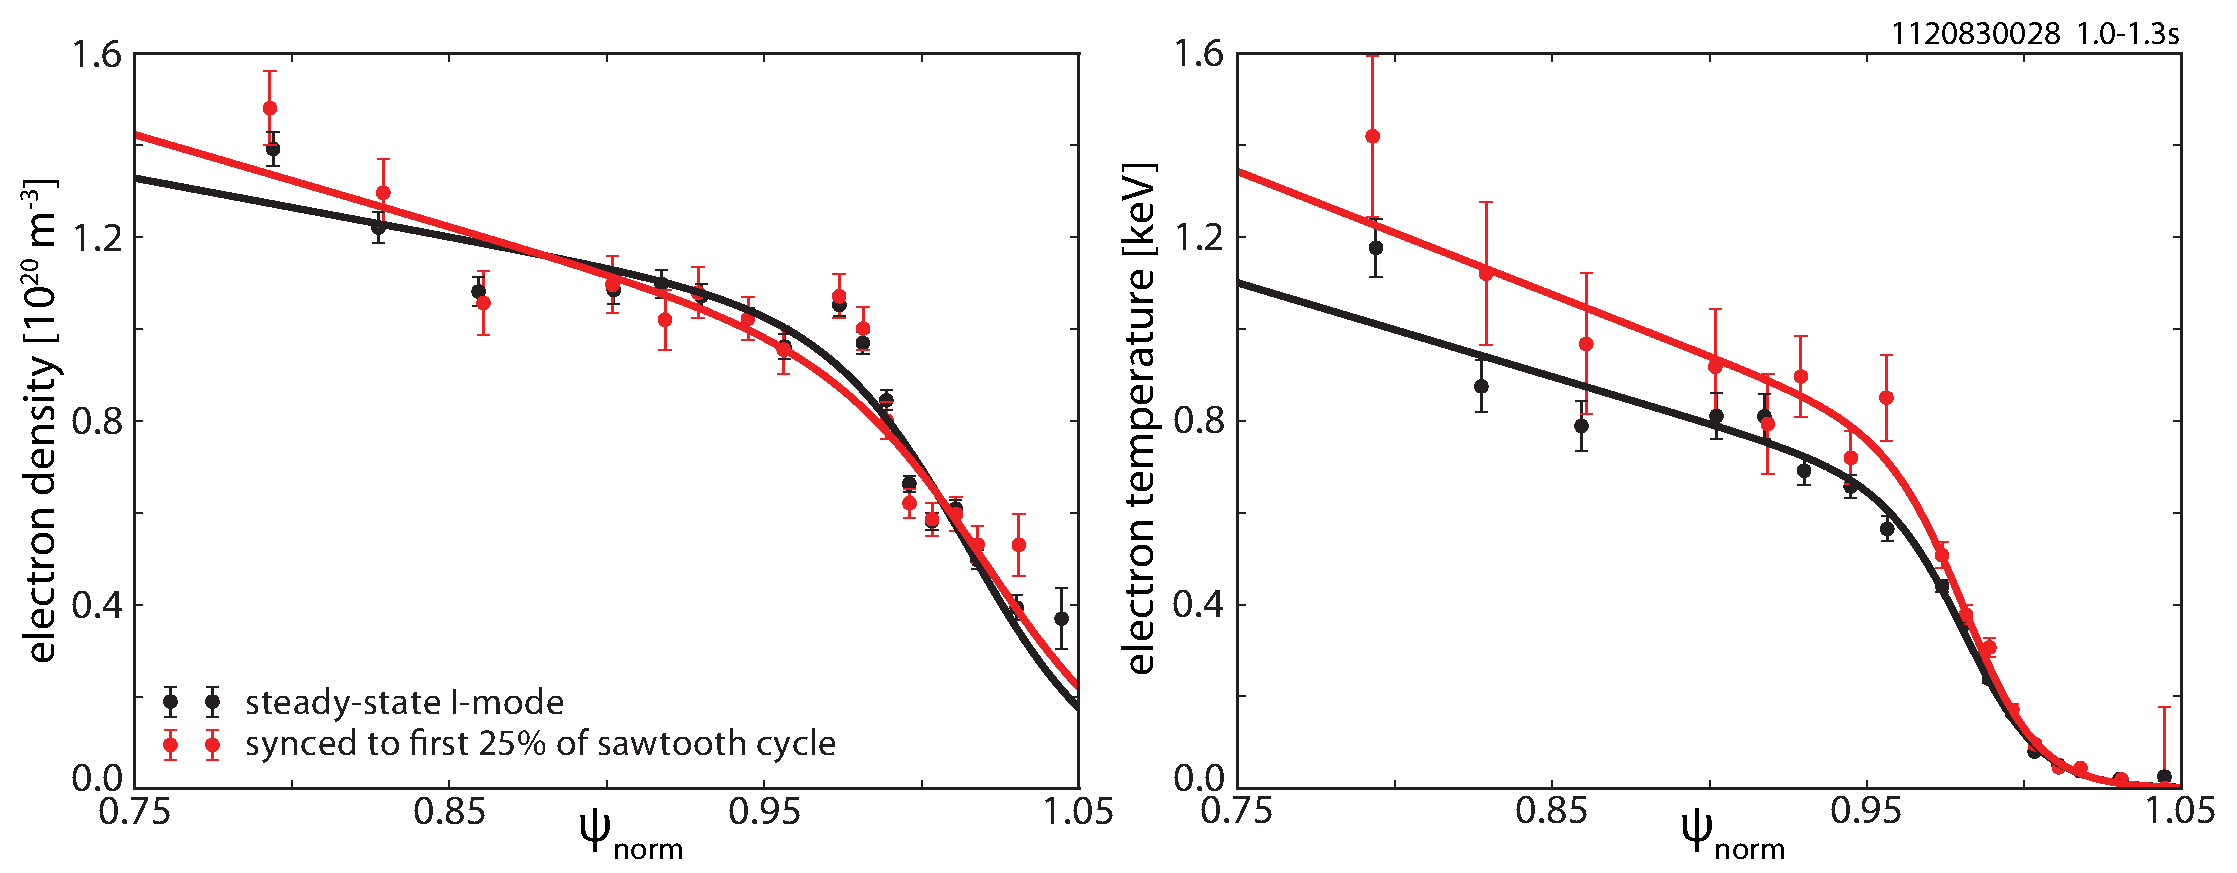
\includegraphics[width=\textwidth]{graphics/IModeModeling/1120830028_prof_stbin.pdf}
 
 \large
 prepare data by masking TS frames to first 25\% of sawtooth cycle (immediately following heat pulse reaching edge) -- similar to ELM-binning technique used for ELMy H-mode

\end{frame}

%%%%%%%%%%%%%%%%%%%%%%%%%%%%%%%%%%%%%%%%%%%%%%%%%%%%%%%%%%%%%%%%%%%%%

\begin{frame}{Sawtooth measurably perturbs pedestal in stability space, but insufficient to reach ELM threshold}

 \centering
 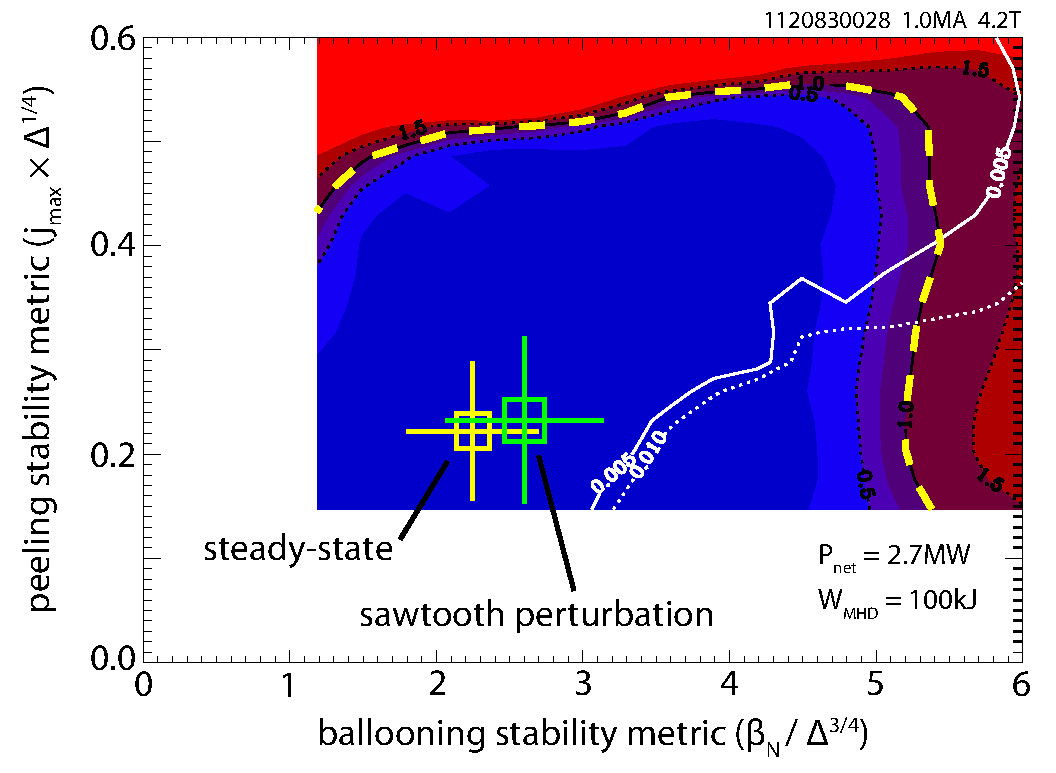
\includegraphics[width=0.8\textwidth]{graphics/IModeModeling/1120830028_stbin_elite.pdf}

\end{frame}

%%%%%%%%%%%%%%%%%%%%%%%%%%%%%%%%%%%%%%%%%%%%%%%%%%%%%%%%%%%%%%%%%%%%%

\begin{frame}{I-mode sawtooth $H_\alpha$ events (mostly) do not exhibit characteristic temperature crash expected for ELMs}

 \centering
 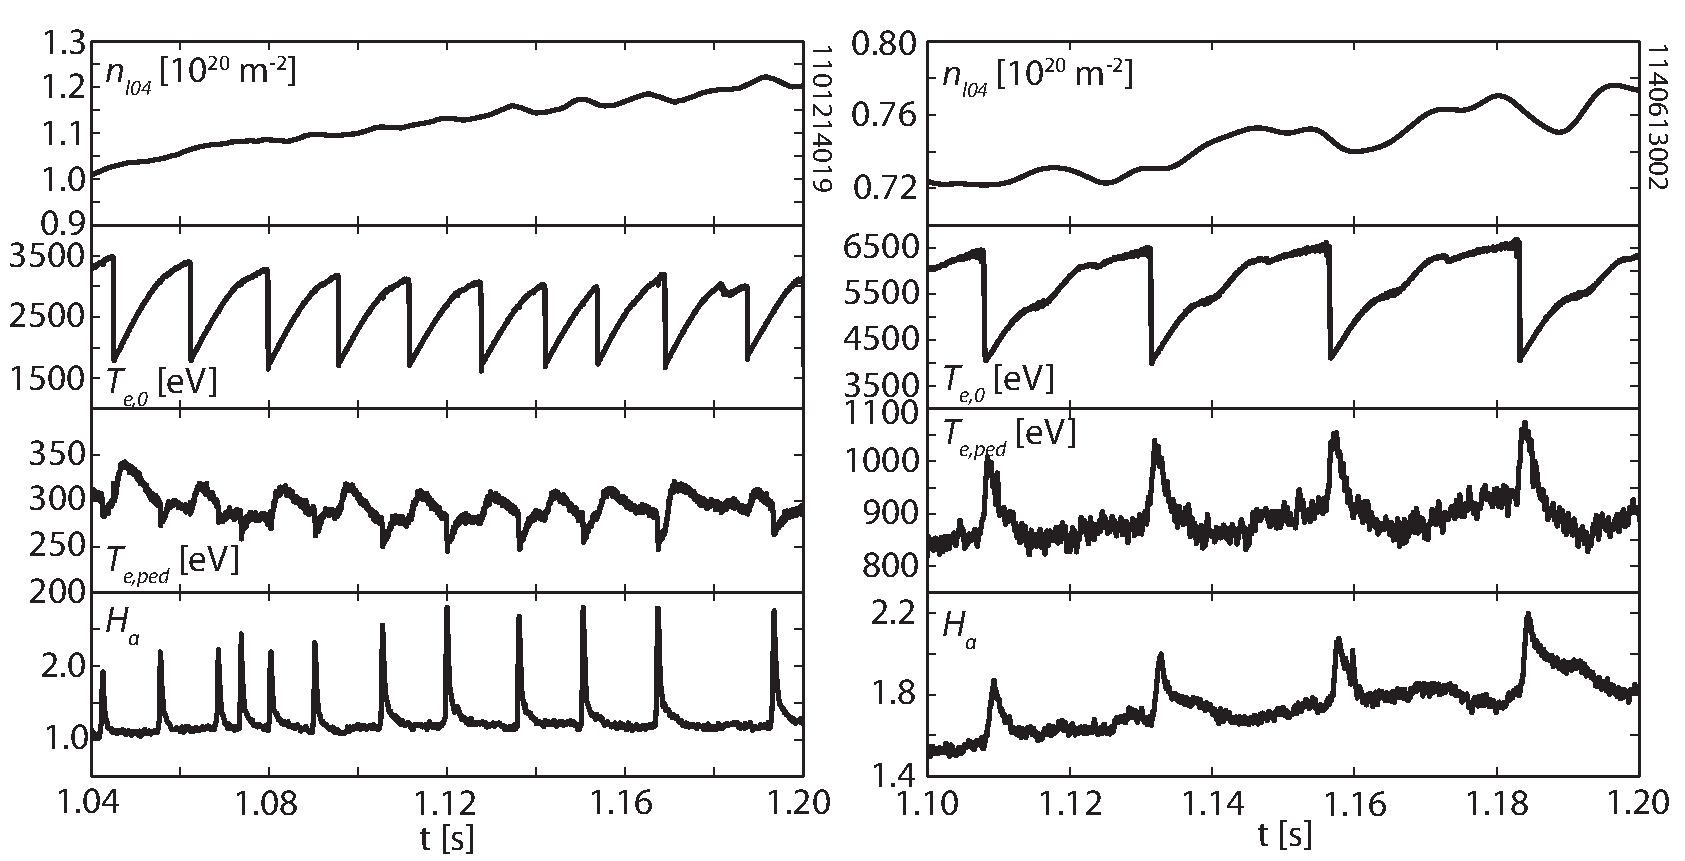
\includegraphics[width=\textwidth]{graphics/IModeModeling/trace_elmy_imode_2.pdf}

\end{frame}

%%%%%%%%%%%%%%%%%%%%%%%%%%%%%%%%%%%%%%%%%%%%%%%%%%%%%%%%%%%%%%%%%%%%%

\begin{frame}{Outline}

 \setbeamercolor{normal text}{fg=gray,bg=}
 \setbeamercolor{alerted text}{fg=black,bg=}
 \usebeamercolor{normal text}

\begin{itemize}
 \large
 \item \textbf{I-Mode Pedestals \& Global Performance}\footnote[2]{JR Walk \emph{et al.}, \emph{Physics of Plasmas} \textbf{21} (2014)}$^,$\footnote[3]{\emph{Invited talk}, APS-DPP Nov. 2013}
 \begin{itemize}
  \large
  \item Pedestal response to fueling, heating power
  \item Pedestal widths and gradients
  \item Global performance and confinement scalings
 \end{itemize}
 \vspace{0.5em}
 \item \textbf{I-Mode Pedestal Stability}
 \begin{itemize}
  \large
  \item P-B MHD, KBM modeling
  \item ELM characterization
 \end{itemize}
 \vspace{0.5em}
 \alert<+>{\item \textbf{Summary, Future Work, \& Questions}}
\end{itemize}

\end{frame}

%%%%%%%%%%%%%%%%%%%%%%%%%%%%%%%%%%%%%%%%%%%%%%%%%%%%%%%%%%%%%%%%%%%%%

\appendix
\newcounter{finalframe}
\setcounter{finalframe}{\value{framenumber}}

\begin{frame}{}

 \begin{center}
  \LARGE{Supplemental Slides}
 \end{center}

 \begin{tikzpicture}[overlay]
  \node[anchor=east,xshift=-2ex,yshift=-20.5ex] at (current page.south east) {\includegraphics[height=2cm]{cmodlogo.eps}};
 \end{tikzpicture}

\end{frame}

%%%%%%%%%%%%%%%%%%%%%%%%%%%%%%%%%%%%%%%%%%%%%%%%%%%%%%%%%%%%%%%%%%%%%

\begin{frame}{Plasma shaping in C-Mod operation}

 \begin{columns}[c]
  \column{0.5\textwidth}
   \centering
   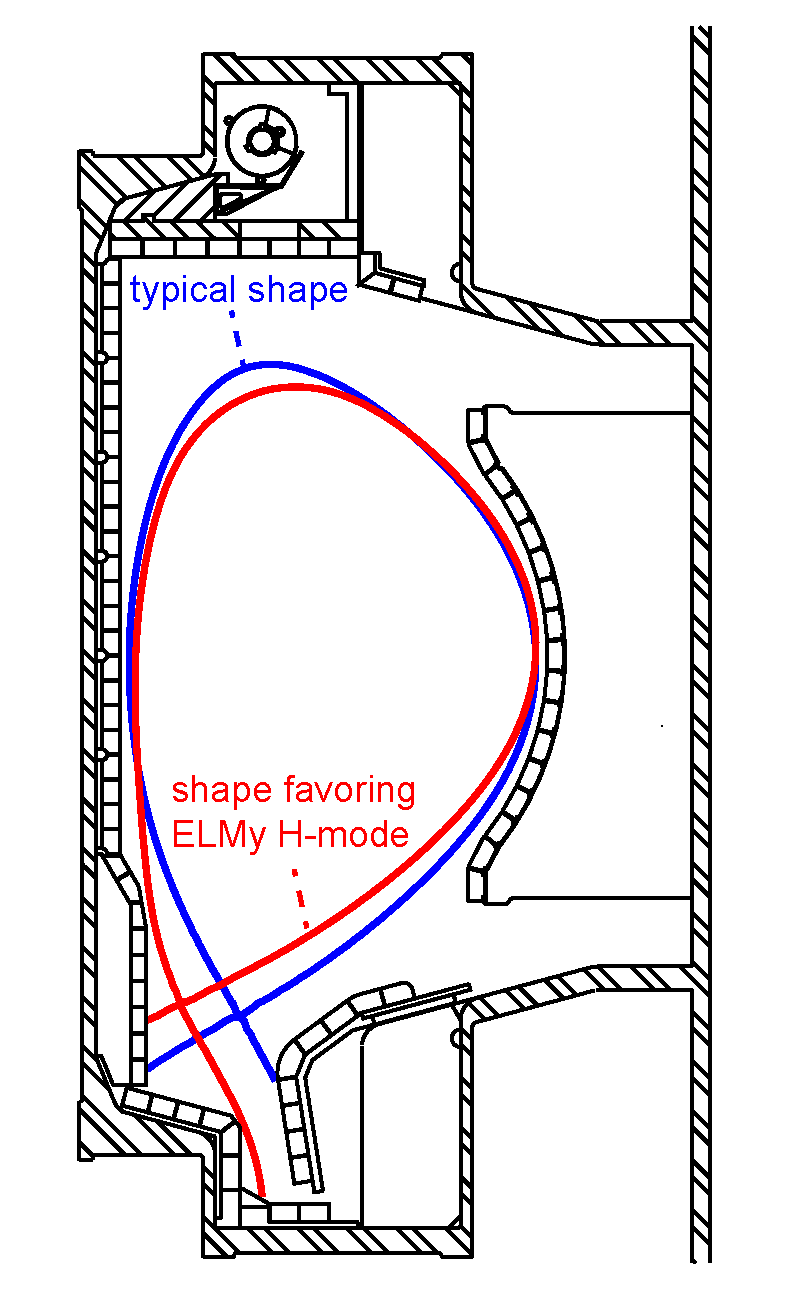
\includegraphics[width=0.8\columnwidth]{graphics/ELMy/shaping.pdf}
  \column{0.5\textwidth}
   \begin{itemize}
    \item I-mode operates at typical shaping for C-Mod plasmas (with reversed $I_p$, $B_T$ for unfavorable $\nabla B$ drift)
    \vspace{0.5em}
    \item ELMy H-mode on C-Mod requires special shaping with low elongation, upper triangularity, high lower triangularity -- in normal shaping in forward field, reach ELM-free H-mode (low $\nu^*$) or EDA H-mode (high $\nu^*$)
   \end{itemize}
 \end{columns}

\end{frame}

%%%%%%%%%%%%%%%%%%%%%%%%%%%%%%%%%%%%%%%%%%%%%%%%%%%%%%%%%%%%%%%%%%%%%

\begin{frame}{Density, temperature, and pressure widths\\ in ELMy H-mode}

 \begin{columns}[c]
  \column{0.5\textwidth}
   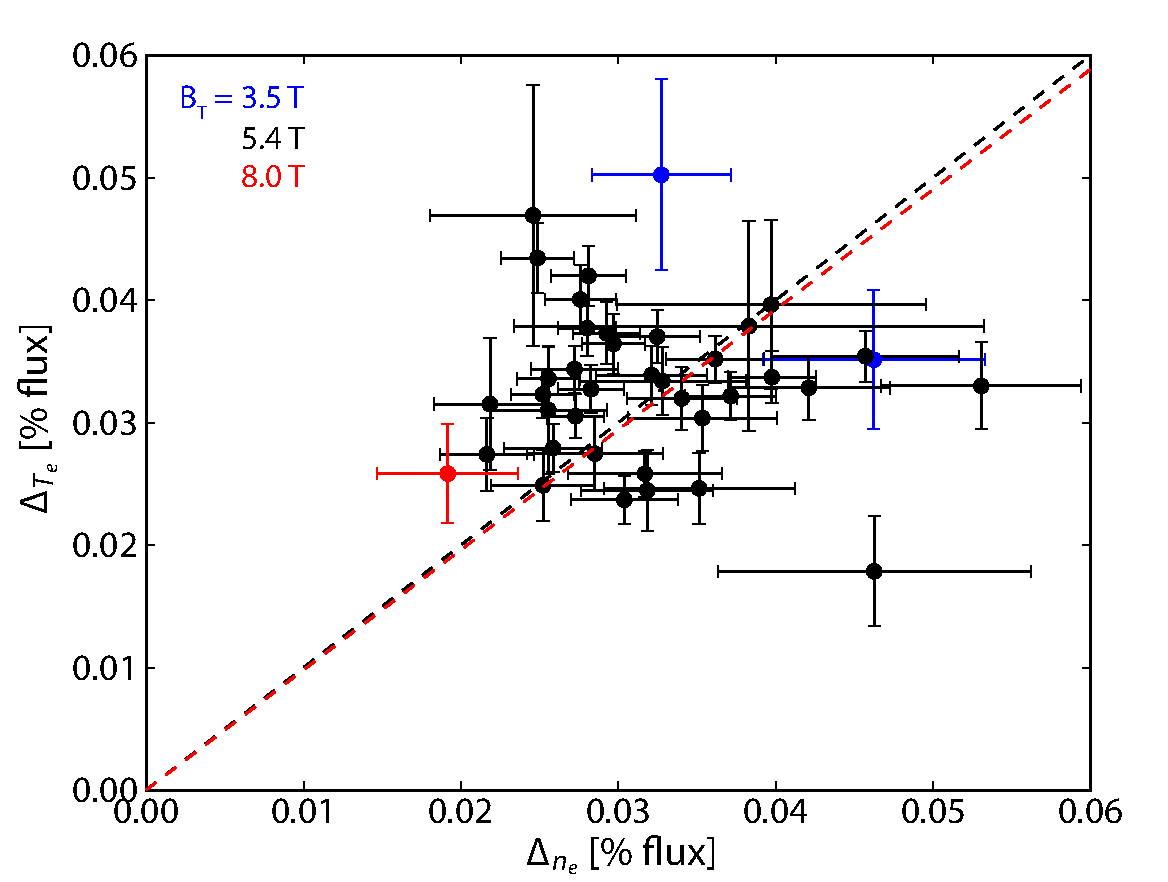
\includegraphics[width=\columnwidth]{graphics/ELMy/deltan_deltaT.pdf}
  \column{0.5\textwidth}
   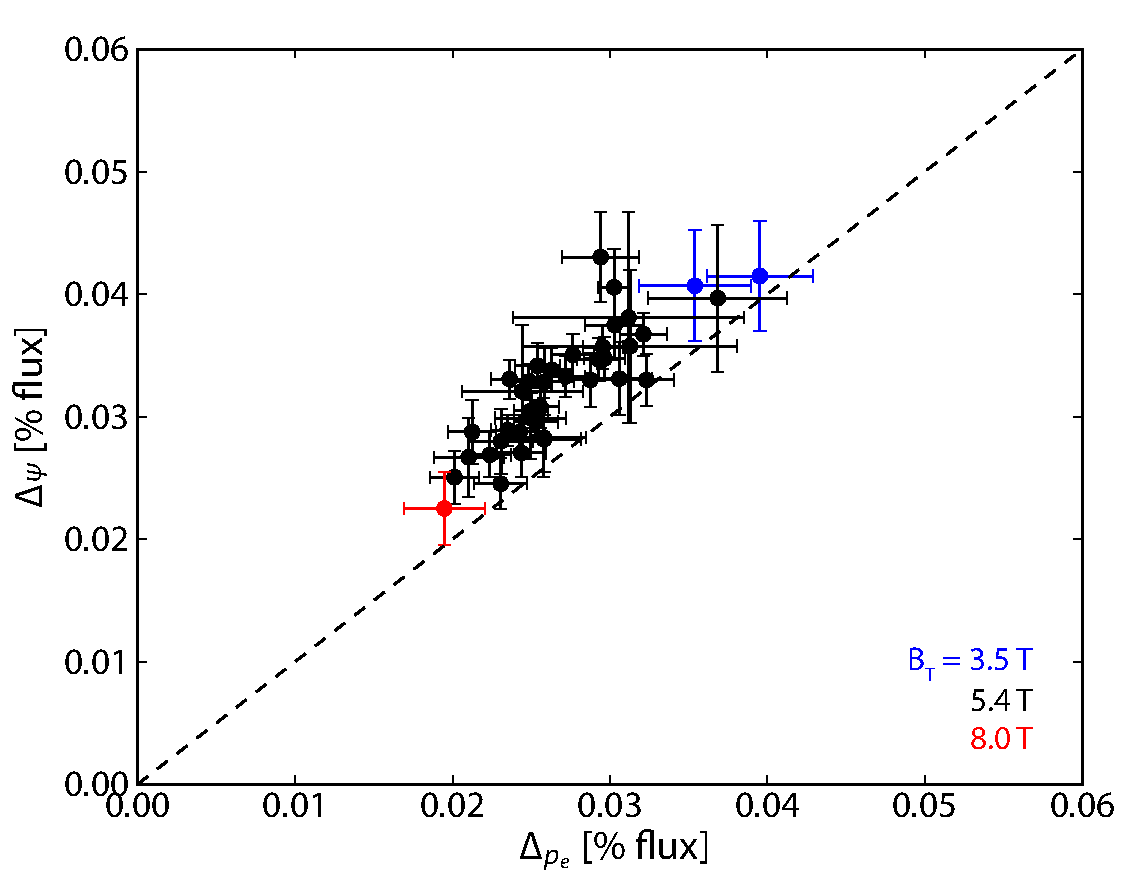
\includegraphics[width=\columnwidth]{graphics/ELMy/deltap_deltapsi.pdf}
 \end{columns}
 
 \large
 \vspace{0.5em}
 $\Delta_\psi = (\Delta_{n_e} + \Delta_{T_e})/2$, tracks with directly-measured $\Delta_{p_e}$

\end{frame}

%%%%%%%%%%%%%%%%%%%%%%%%%%%%%%%%%%%%%%%%%%%%%%%%%%%%%%%%%%%%%%%%%%%%%

\begin{frame}{$\beta_{p,95}$ scaling with norm. density in addition to heating-power response}

 \begin{columns}[c]
  \column{0.4\textwidth}
   \begin{itemize}
    \large
    \item $P_{net}/\overline{n}_e$ sets slope of $T_e/B_p$ line -- response of pedestal temperature at fixed current
    \vspace{0.5em}
    \item pressure responds to fueling, provided sufficient power to maintain the pedestal
   \end{itemize}
  \column{0.6\textwidth}
   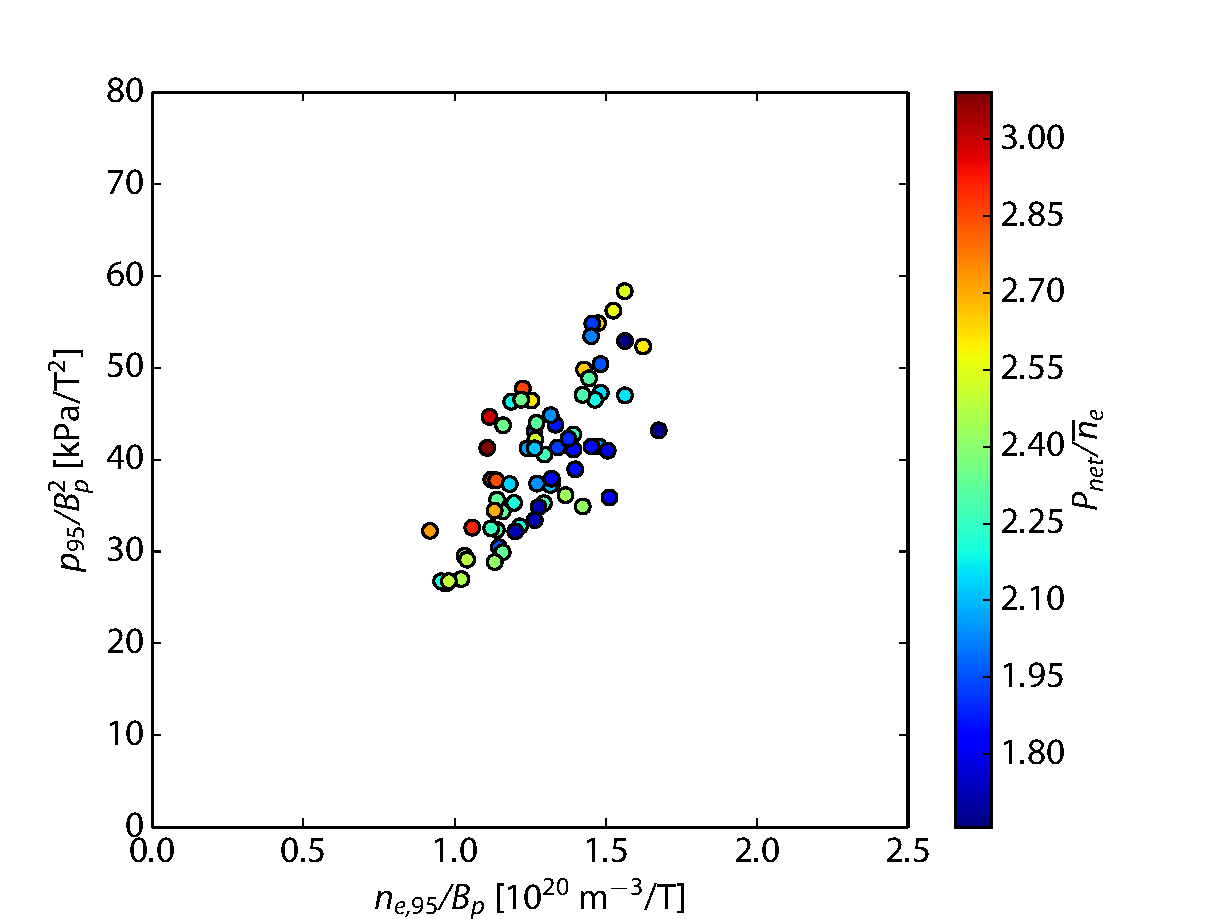
\includegraphics[width=\columnwidth]{graphics/IModeModeling/neBp_pBp_Pnebar.pdf}
 \end{columns}

\end{frame}

%%%%%%%%%%%%%%%%%%%%%%%%%%%%%%%%%%%%%%%%%%%%%%%%%%%%%%%%%%%%%%%%%%%%%

\begin{frame}

\large
\begin{equation*}
 \begin{aligned}
  \vec{Q} &= \nabla \times \left( \vec{\xi} \times \vec{B} \right)\\
  \delta W &= \delta W_F + \delta W_S + \delta W_V\\
  \delta W_F &= \frac{1}{2} \int_P d^3 \vec{r} \Bigg[ \frac{|\vec{Q}|^2}{\mu_0} + \frac{B^2}{\mu_0} \left| \nabla \cdot \vec{\xi}_\perp + 2 \vec{\xi}_\perp \cdot \vec{\kappa} \right|^2 + \gamma p \left| \nabla \cdot \vec{\xi} \right|^2\\
  &\quad- 2\left( \vec{\xi}_\perp \cdot \nabla p \right) \left(\vec{\kappa} \cdot \vec{\xi}_\perp^* \right) - j_\parallel \left(\vec{\xi}_\perp^* \times \vec{b} \right) \cdot \vec{Q}_\perp \Bigg]\\
  \delta W_S &= \frac{1}{2} \int_S dS \left| \hat{n} \cdot \vec{\xi}_\perp \right|^2 \hat{n} \cdot \left[ \nabla \left( p + \frac{B^2}{2\mu_0} \right) \right]\\
  \delta W_V &= \frac{1}{2} \int_V d^3 \vec{r} \frac{\left|B_1 \right|^2}{\mu_0}
 \end{aligned}
\end{equation*}

\end{frame}

%%%%%%%%%%%%%%%%%%%%%%%%%%%%%%%%%%%%%%%%%%%%%%%%%%%%%%%%%%%%%%%%%%%%%

\begin{frame}

\large
\begin{equation*}
 \begin{aligned}
  X &= RB_p \xi_\psi\\
  ik_\parallel &= \frac{1}{JB} \left( \frac{\partial}{\partial \chi} + in \nu \right) \qquad \nu = JB_T/R\\
  P &= \sigma X + \frac{B_p^2}{\nu B^2} \frac{F}{n} \frac{\partial}{\partial \psi} \left( JBk_\parallel \right)\\
  Q &= \frac{X}{B^2} \frac{dp}{d\psi} + \frac{F^2}{\nu R^2 B^2} \frac{1}{n} \frac{\partial}{\partial \psi} \left( JBk_\parallel X \right)\\
  \sigma &= -\frac{F}{B^2} \frac{dp}{d\psi} - \frac{dF}{d\psi} = -\frac{j_\parallel}{B}
 \end{aligned}
\end{equation*}

\end{frame}

%%%%%%%%%%%%%%%%%%%%%%%%%%%%%%%%%%%%%%%%%%%%%%%%%%%%%%%%%%%%%%%%%%%%%

\begin{frame}

 \large
 \begin{equation*}
 \begin{aligned}
  \delta W &= \pi \iint d\psi d\chi \Bigg\{ \frac{JB^2}{R^2 B_p^2} \left| k_\parallel X \right|^2 + \frac{R^2 B_p^2}{JB^2} \left| \frac{1}{n} \frac{\partial}{\partial \psi} \left( JB k_\parallel X \right) \right|^2\\
  &\quad- \frac{2J}{B^2} \frac{dp}{d\psi} \left[ \left| X \right|^2 \frac{\partial}{\partial \psi} \left( p + \frac{B^2}{2} \right) - \frac{iF}{JB^2} \frac{\partial}{\partial \chi} \left( \frac{B^2}{2} \right) \frac{X^*}{n} \frac{\partial X}{\partial \psi} \right]\\
  &\quad-\frac{X^*}{n} JBk_\parallel \left( X \frac{d\sigma}{d\psi} \right) + \frac{1}{n} \left[ PJBk_\parallel^* Q^* + P^* JBk_\parallel Q \right]\\
  &\quad+ \frac{\partial}{\partial \psi} \left[ \frac{\sigma}{n} X^* JBk_\parallel X \right] \Bigg\}
 \end{aligned}
\end{equation*}

\end{frame}

%%%%%%%%%%%%%%%%%%%%%%%%%%%%%%%%%%%%%%%%%%%%%%%%%%%%%%%%%%%%%%%%%%%%%

\setcounter{framenumber}{\value{finalframe}}

\end{document}